\documentclass[11pt]{article}
\def\DoNotLoadEpstopdf{}
\usepackage[T1]{fontenc}
\usepackage{lmodern}
\usepackage[margin=1in]{geometry}
\usepackage{amsmath,amssymb,amsthm,mathtools}
\usepackage{enumitem,microtype,xcolor,tikz}
\usepackage[nottoc]{tocbibind}
\usepackage[colorlinks=true,linkcolor=blue!45!black,citecolor=blue!45!black,urlcolor=blue!45!black]{hyperref}
\hypersetup{pdftitle={Constant-factor hardness of Min-UnCut},pdfauthor={OpenAI}}
\pdfinfoomitdate=1
\pdftrailerid{}
\pdfsuppressptexinfo=15

\pdfgentounicode=1
\pdfglyphtounicode{tfm:lmex10/parenleftbig}{0028}
\pdfglyphtounicode{tfm:lmex10/parenleftBig}{0028}
\pdfglyphtounicode{tfm:lmex10/parenleftbigg}{0028}
\pdfglyphtounicode{tfm:lmex10/parenleftBigg}{0028}
\pdfglyphtounicode{tfm:lmex10/parenrightbig}{0029}
\pdfglyphtounicode{tfm:lmex10/parenrightBig}{0029}
\pdfglyphtounicode{tfm:lmex10/parenrightbigg}{0029}
\pdfglyphtounicode{tfm:lmex10/parenrightBigg}{0029}
\pdfglyphtounicode{tfm:lmex10/bracketleftbig}{005B}
\pdfglyphtounicode{tfm:lmex10/bracketrightbig}{005D}
\pdfglyphtounicode{tfm:lmex10/ceilingleftbigg}{2308}
\pdfglyphtounicode{tfm:lmex10/ceilingrightbigg}{2309}
\pdfglyphtounicode{tfm:lmex10/braceleftBigg}{007B}
\pdfglyphtounicode{tfm:lmex10/bracerightBigg}{007D}
\pdfglyphtounicode{tfm:lmex10/vextendsingle}{23D0}
\pdfglyphtounicode{tfm:lmex10/bracketlefttp}{23A1}
\pdfglyphtounicode{tfm:lmex10/bracketrighttp}{23A4}
\pdfglyphtounicode{tfm:lmex10/bracketleftbt}{23A3}
\pdfglyphtounicode{tfm:lmex10/bracketrightbt}{23A6}
\pdfglyphtounicode{tfm:lmex10/summationtext}{2211}
\pdfglyphtounicode{tfm:lmex10/summationdisplay}{2211}
\pdfglyphtounicode{tfm:lmex10/producttext}{220F}
\pdfglyphtounicode{tfm:lmex10/productdisplay}{220F}
\pdfglyphtounicode{tfm:lmex10/integraltext}{222B}
\pdfglyphtounicode{tfm:lmex10/integraldisplay}{222B}
\pdfglyphtounicode{tfm:lmex10/radicalbig}{221A}
\pdfglyphtounicode{tfm:lmex10/radicalBig}{221A}
\pdfglyphtounicode{tfm:lmex10/radicalBigg}{221A}
\pdfglyphtounicode{tfm:lmex10/hatwide}{0302}
\pdfglyphtounicode{tfm:lmex10/hatwider}{0302}
\pdfglyphtounicode{tfm:msbm10/hatwider}{0302}
\pdfglyphtounicode{tfm:lmmi10/mu}{03BC}
\pdfglyphtounicode{tfm:lmmi8/mu}{03BC}
\pdfglyphtounicode{tfm:lmsy10/openbullet}{2218}
\pdfglyphtounicode{tfm:lmsy10/backslash}{2216}
\pdfglyphtounicode{tfm:lmsy8/backslash}{2216}
\pdfglyphtounicode{tfm:lmsy6/backslash}{2216}
\pdfglyphtounicode{tfm:lmsy10/bardbl}{2016}
\pdfglyphtounicode{tfm:msbm10/E}{1D53C}
\pdfglyphtounicode{tfm:msbm10/F}{1D53D}
\pdfglyphtounicode{tfm:msbm10/P}{2119}
\pdfglyphtounicode{tfm:msbm10/Q}{211A}
\pdfglyphtounicode{tfm:msbm10/R}{211D}
\pdfglyphtounicode{tfm:lmsy10/C}{1D49E}
\pdfglyphtounicode{tfm:lmsy10/E}{2130}
\pdfglyphtounicode{tfm:lmsy10/F}{2131}
\pdfglyphtounicode{tfm:lmsy10/K}{1D4A6}
\pdfglyphtounicode{tfm:lmsy10/L}{2112}
\pdfglyphtounicode{tfm:lmsy10/R}{211B}
\pdfglyphtounicode{tfm:lmsy8/C}{1D49E}
\pdfglyphtounicode{tfm:lmsy8/K}{1D4A6}
\pdfglyphtounicode{tfm:lmsy8/R}{211B}
\pdfglyphtounicode{tfm:eufm10/d}{1D521}
\pdfglyphtounicode{tfm:lmmib10/alpha}{1D736}
\pdfglyphtounicode{tfm:rm-lmbx10/one}{1D7CF}
\setlength{\emergencystretch}{2em}
\numberwithin{equation}{section}
\newtheorem{theorem}{Theorem}[section]
\newtheorem{lemma}[theorem]{Lemma}
\newtheorem{proposition}[theorem]{Proposition}
\newtheorem{corollary}[theorem]{Corollary}
\theoremstyle{definition}
\newtheorem{definition}[theorem]{Definition}
\theoremstyle{remark}
\newtheorem{remark}[theorem]{Remark}
\newcommand{\F}{\mathbb F}
\newcommand{\R}{\mathbb R}
\newcommand{\N}{\mathbb N}
\newcommand{\E}{\mathbb E}
\newcommand{\Prob}{\mathbb P}
\newcommand{\C}{\mathcal C}
\newcommand{\D}{\mathcal D}
\newcommand{\one}{\mathbf 1}
\newcommand{\eps}{\varepsilon}
\newcommand{\TV}{\operatorname{TV}}
\newcommand{\val}{\operatorname{val}}
\newcommand{\OPT}{\operatorname{OPT}}
\newcommand{\sgn}{\operatorname{sgn}}
\newcommand{\supp}{\operatorname{supp}}
\newcommand{\im}{\operatorname{im}}
\newcommand{\rank}{\operatorname{rank}}
\newcommand{\Cost}{\operatorname{Cost}}
\newcommand{\Uncut}{\operatorname{uncut}}
\newcommand{\poly}{\operatorname{poly}}
\newcommand{\NP}{\mathsf{NP}}
\newcommand{\RP}{\mathsf{RP}}
\newcommand{\norm}[1]{\lVert#1\rVert}
\newcommand{\abs}[1]{\lvert#1\rvert}
\newcommand{\ip}[2]{\langle#1,#2\rangle}
\newcommand{\dd}{\,\mathrm d}
\title{Constant-factor hardness of Min-UnCut}
\author{OpenAI}
\date{September 23, 2026}
\begin{document}
\maketitle
\begin{abstract}
For every fixed \(C>1\), approximating Min-UnCut within factor \(C\) is
NP-hard, even on simple undirected unweighted graphs.
\end{abstract}
\tableofcontents
\section{Introduction}
\label{sec:introduction}

For a finite simple undirected graph $G=(V,E)$ and a bipartition
$V=S\sqcup(V\setminus S)$, define
\[
 \Uncut_G(S)=\abs{\{uv\in E:u,v\in S\text{ or }u,v\notin S\}},
 \qquad
 \OPT_{\rm uncut}(G)=\min_{S\subseteq V}\Uncut_G(S).
\]
The two parts may be empty and need not be balanced. Equivalently,
$\OPT_{\rm uncut}(G)$ is the minimum number of edges whose deletion makes
$G$ bipartite: deleting the uncut edges of a partition suffices, and a
bipartition of any remaining bipartite graph makes every uncut edge belong
to the deleted set. This is the edge-deletion problem throughout.

Min-UnCut measures distance from bipartiteness. Although its objective is the
number of edges minus the maximum cut size, a multiplicative approximation
for Max-Cut does not give a comparable multiplicative approximation for
Min-UnCut when the graph is nearly bipartite. Its approximation question
therefore concerns how accurately one can recognize and exploit that regime.
Agarwal, Charikar, Makarychev and Makarychev gave a randomized polynomial-time
$O(\sqrt{\log |V|})$ approximation for Min-UnCut~\cite[Theorem~2.1]{ACMM2005}.
Under the Unique Games Conjecture, the near-satisfiable Max-Cut gap of
Khot, Kindler, Mossel and O'Donnell implies arbitrarily large constant
gaps for weighted Min-UnCut~\cite{KKMO2007}: graphs admitting a cut that
misses at most an $\eta$ fraction of the total edge weight are hard to
distinguish from graphs in which every cut misses a constant times
$\sqrt\eta$ of that weight. The ratio of these two
uncut costs grows without bound as $\eta$ decreases.

Unconditional lower bounds for particular constants have developed through
successively stronger finite gadgets. H\aa stad, Huang, Manokaran,
O'Donnell and Wright proved hardness for every factor below $11/8$ in the
weighted minimum-deletion formulation of Max-Cut
\cite[Corollary~3.3]{HHMOW2017}. Wiman strengthened the near-satisfiable
Max-Cut gap to give factors below $1.45685$~\cite[Theorem~3.18]{Wiman2018}.
Martinsson subsequently obtained hardness for every factor below
$73139148/49096883\approx1.48969$ for minimizing the weight of violated
two-variable parity equations~\cite[Theorem~1.1]{Martinsson2024}.
The last result transfers to weighted Min-UnCut by replacing equality and
inequality constraints by paths of lengths four and three, respectively,
with fresh internal vertices and the constraint's weight on each edge.
For fixed endpoint bits each path has minimum uncut weight equal to the
violated constraint's weight, so this preserves absolute minimum cost even
though the total weight changes. These results concern individual constant
factors; the theorem below gives every prescribed constant factor on simple
unweighted graphs.

\begin{theorem}\label{thm:main}
For every fixed integer $K\ge2$, there is a deterministic polynomial-time
many-one reduction mapping a $3$SAT formula $\varphi$ to a pair $(G,k)$, where
$G$ is an explicit finite simple undirected unweighted graph and $k\ge1$ is
a binary-encoded integer, such that
\[
 \begin{aligned}
 \varphi\text{ satisfiable}&\quad\Longrightarrow\quad
       \OPT_{\rm uncut}(G)\le k,\\
 \varphi\text{ unsatisfiable}&\quad\Longrightarrow\quad
       \OPT_{\rm uncut}(G)>Kk.
 \end{aligned}
\]
For each fixed $K$, the graph size, full construction work, and bit complexity
are polynomial in the bit length of $\varphi$. All constants are effective;
no advice or oracle is supplied to the reduction.
\end{theorem}

Theorem~\ref{thm:main} resolves the constant-factor approximability question
for Min-UnCut in the hardness direction. It assumes neither the Unique Games
Conjecture nor any other unproved hardness hypothesis. Choosing an integer
$K$ at least any prescribed real factor $C>1$ shows that a deterministic
polynomial-time $C$-approximation would imply $\mathsf P=\NP$.
The positive threshold $k$ separates this assertion from ordinary
bipartiteness testing. For a randomized approximation with constant success
probability, the corresponding consequence is $\NP\subseteq\RP$;
Section~\ref{sec:finite} explains the one-sided test.

In minimum $2$CNF clause deletion, the input is an explicit list of
two-literal disjunctions, each of unit cost, and one deletes as few clause
occurrences as possible to make the remaining formula satisfiable. Write
$\OPT_{\rm del}(F)$ for this minimum and $\operatorname{unsat}(F,a)$ for the
number of clause occurrences falsified by an assignment $a$. Agarwal et al.
also give a randomized polynomial-time $O(\sqrt{\log n})$ approximation
for this problem on $n$ variables~\cite[Theorem~3.1]{ACMM2005}.

\begin{corollary}\label{cor:min-2cnf-deletion}
For every fixed real $C>1$, minimum $2$CNF clause deletion is NP-hard to
approximate within factor $C$. In particular, a deterministic polynomial-time
$C$-approximation would imply $\mathsf P=\NP$.
\end{corollary}

The proof in Section~\ref{sec:2cnf-consequence} replaces each edge by two
clauses and preserves the optimum deletion cost exactly.

\subsection{Proof strategy}

The reduction first constructs weighted comparisons between bits using
Gaussian-sampled queries. A satisfying source instance admits bits of total comparison
cost at most $4$, whereas an unsatisfiable instance forces cost greater than
an arbitrarily prescribed constant $J$. The graph construction then realizes
each failed comparison by exactly one uncut edge. The main work is obtaining
this comparison gap with constants chosen before the label alphabet.

\paragraph{A game with affine labels.}
The starting point is H\aa stad's near-satisfiable gap for three-variable
parity equations~\cite{Hastad2001}, recalled with ordinary parallel
repetition in Section~\ref{sec:preliminaries}. A first player receives a tuple
of equations and labels it by satisfying assignments to the separate
equations. A second player sees the full equations in most coordinates and
only a queried variable in a small set of hidden coordinates. Its label
supplies the corresponding bits. The verifier checks agreement. The two
label sets are finite affine spaces over $\F_2$, and agreement is an affine
map from the first space to the second.

Section~\ref{sec:outer} proves two properties of this game. Its soundness
survives giving both players a fixed number of shared affine functions on
their labels: many hidden coordinates have zero coefficients in all those
functions and still support ordinary repetition. Also, a fixed number of
uniform affine functions on the second alphabet, pulled back through the
random agreement map, have joint distribution close to independent uniform
functions on the first alphabet. The latter is a statement about the whole
collection; it allows later decoding choices to depend on some of its
members. These properties are proved directly for the questions used here.

\paragraph{A comparison test for arbitrary bit proofs.}
At each question with alphabet $A$, replace a label $a$ by a function
$f$ assigning a sign $f(P)\in\{1,-1\}$ to every Boolean query
$P:A\to\{1,-1\}$. The intended function evaluates
queries, $f(P)=P(a)$. Arbitrary functions are required only to satisfy
$f(-P)=-f(P)$, the usual folding relation. We must extract labels from
arbitrary such functions whose comparison cost is small.

Section~\ref{sec:inner-smoothing} constructs three tests using random affine
functions and Gaussian thresholds. The affine functions are arranged on
$X=[n]^m$ as sums of $m$ arrays, with the $i$th array independent of the
$i$th coordinate. Each test compares two queries obtained by a controlled
change of this data. The tests respectively control Gaussian perturbations,
resampling of array entries, and changes in individual entries of a Boolean
truth table. Evaluation proofs have small cost in all three tests.

For a general proof, Gaussian averaging gives a smooth real-valued function
of the threshold parameters. Its gradient retains nonzero energy because
the first test rarely changes the answer. The other two tests control its
Fourier degrees and its correlation with products of functions each missing
one coordinate of $X$. These bounds use the number of array positions,
not the number of affine labels.

\paragraph{Extracting a label without an alphabet-size loss.}
Section~\ref{sec:inner-box} converts that correlation into a large Fourier
coefficient in one affine-function entry, with all other entries fixed.
The coefficient is odd: its character changes sign upon adding the constant
function $1$. Each such character has the form $b\mapsto(-1)^{b(a)}$ for a unique
label $a$, by Lemma~\ref{lem:odd-labels}.

The extraction uses symmetries of the array representation to pair equal
odd frequencies. Restricting to a random smaller box then separates their
remaining random variables. Repeated Cauchy--Schwarz removes the arbitrary
functions missing coordinates and leaves products over cube vertices.
The terms involving the Gaussian coordinate at the tested point vanish by
centering, while the paired terms factor over independent four-corner
squares, each controlled by a Fourier coefficient. The selection of terms depends only on which
array entries and Gaussian degrees occur; it never enumerates label
frequencies. This distinction gives an extraction probability and
coefficient size independent of the affine alphabet.

\paragraph{Composition and finite graphs.}
Section~\ref{sec:composition} adds a fourth test comparing the two players'
answers to the same pulled-back query. Low cost makes their smoothed
one-entry functions close. The large coefficients on each side form short
label lists. Joint approximation of the affine-function distributions
controls the remaining small coefficients through a fourth-moment
identity, even when the first list was chosen using shared background
functions. The lists yield an agreeing pair with fixed positive probability,
contradicting the game's soundness. All inner constants are fixed before
the game's repetition parameters and alphabet.

Finally, Section~\ref{sec:finite} approximates the complete joint Gaussian
sign tables by a rational law. Enumerating this law gives a deterministic
comparison system with polynomial numerical multiplicities for fixed $K$.
Fresh paths of lengths four and three realize equality and inequality
demands exactly, including demands with coincident endpoints. Their costs
have no additive baseline, so a positive integer threshold preserves the
strict multiplicative gap. The constants may be large; the approximation
factor is fixed before the input formula is given.

\subsection{Relation to earlier methods}

The parity-equation starting point belongs to the PCP approach to hardness
of approximation: a locally checked proof gives a finite constraint system
with a gap between satisfiable and unsatisfiable inputs. H\aa stad's
construction provides the near-satisfiable parity gap used here, while the
parallel repetition theorems of Raz and Holenstein amplify the
corresponding two-player game~\cite{Hastad2001,Raz1998,Holenstein2009}.
Neither step assumes Unique Games. In particular, the completeness error
is positive and is selected only after the repetitions have been fixed.

Our bit proofs use the long code and folding of Bellare, Goldreich and
Sudan~\cite{BGS1998}, which also underlie H\aa stad's Fourier analysis.
Khot and Safra use smooth equation--variable games and decode short label
lists from large Fourier coefficients
\cite[Sections~3.2--3.4 and~5.2]{KS13}.
Shared linear advice and coordinates on which that advice vanishes appear
in Khot, Minzer and Safra~\cite[Sections~3.3--3.4]{KMS17}; a related
shared-subspace formulation appears in Dinur et al.
\cite[Lemma~5.4]{DKKMS2025}.
Our outer-game proofs retain this mechanism but establish the precise
hinted soundness and joint approximation estimates needed by a decoder
that depends on its shared background.

The analytic tools also have established precedents. The Gaussian sign
identity is the random-hyperplane calculation of Goemans and
Williamson~\cite{GW95}, and Gaussian smoothing and Hermite expansions
are standard in noise-stability analysis~\cite{MOO10}. The box estimate
uses the iterated Cauchy--Schwarz mechanism in Gowers's hypergraph
arguments~\cite{Gowers2007}. We prove the identities and inequalities
used here. The additional argument is the extraction of an odd one-entry
coefficient from an arbitrary bit proof, uniformly in its alphabet,
and its transfer through a random affine map when the remaining
coefficients depend on the background.


\section{Preliminaries and unconditional starting theorems}
\label{sec:preliminaries}

All finite-set averages and Fourier transforms use probability normalization.
Every affine space in the paper is a finite nonempty affine space over $\F_2$.
Constants described as fixed are independent of the input instance; their
dependence on the requested approximation factor is allowed.

\subsection{Affine alphabets and odd characters}

For an affine space $A$, let $D(A)$ be the vector space of affine functions
$A\to\F_2$, including constants. If $A$ has dimension $r$, then $D(A)$ has
dimension $r+1$. Write $1\in D(A)$ for the constant-one function. A frequency
is an element $\alpha$ of the linear dual $D(A)^*$, with character
$\chi_\alpha(b)=(-1)^{\alpha(b)}$. Call $\alpha$ \emph{odd} if $\alpha(1)=1$.

\begin{lemma}[Odd frequencies are labels]\label{lem:odd-labels}
The map $a\mapsto\operatorname{ev}_a$, where
$\operatorname{ev}_a(b)=b(a)$, is a bijection from $A$ onto the odd frequencies
of $D(A)$. If $\pi:A\to A'$ is affine and
$\pi^*:D(A')\to D(A)$ is pullback, then its dual sends
$\operatorname{ev}_a$ to $\operatorname{ev}_{\pi(a)}$.
\end{lemma}
\begin{proof}
Choose affine coordinates $A=\F_2^r$. Every affine function is
$b(x)=b_0+\sum_{j=1}^r b_jx_j$. A functional taking the constant function to
one is uniquely $b\mapsto b_0+\sum_j b_ja_j$, for some $a\in\F_2^r$.
Finally $(\pi^*)^*(\operatorname{ev}_a)(b)=b(\pi(a))$.
\end{proof}

For a real function $v$ on a finite binary vector space $W$, write
\[
 \widehat v(\alpha)=\E_{w\in W}v(w)(-1)^{\alpha(w)},\qquad
 v(w)=\sum_{\alpha\in W^*}\widehat v(\alpha)(-1)^{\alpha(w)}.
\]
Character orthogonality gives Parseval's identity
$\sum_\alpha\abs{\widehat v(\alpha)}^2=\E v^2$.
If $T:W'\to W$ is linear, each character of $v$ pulls back to its image
under $T^*$; coefficients with the same image add. Injectivity and
surjectivity of $T$ are unnecessary. We will use the identity
\begin{equation}\label{eq:fourth-moment}
 \sum_\alpha\abs{\widehat v(\alpha)}^4
 =\E_{a,b,c\in W}v(a)v(b)v(c)v(a+b+c).
\end{equation}
Indeed, expansion of the four factors and averaging over the three independent
points force all four frequencies to agree.

\subsection{Gaussian identities}

We recall the Fourier--Hermite identities used in Gaussian
noise-stability analysis~\cite[Sections~4.1 and~5]{MOO10}, with proofs of the needed forms.
Let $\gamma_d$ be standard Gaussian probability measure on $\R^d$. The normalized
Hermite polynomials $H_j$ are specified by
\[
 e^{tz-t^2/2}=\sum_{j\ge0}H_j(z)\frac{t^j}{\sqrt{j!}}.
\]
Gaussian integration of the product of two generating functions proves their
orthonormality. Their products
$\psi_I(c)=\prod_x H_{I_x}(c_x)$ form an orthonormal basis of
$L^2(\gamma_d)$. For completeness, if a function is orthogonal to all these
polynomials, its Gaussian-weighted exponential transform has every Taylor
coefficient zero. Cauchy--Schwarz makes that transform entire in each variable;
its restriction to imaginary arguments is the Fourier transform of an
integrable function, which is therefore zero. Thus the original function is
zero almost everywhere.

Differentiating the generating function gives
$H_j'=\sqrt j H_{j-1}$. Consequently, for a function with square-integrable
weak gradient,
\begin{equation}\label{eq:hermite-energy}
 \int\norm{\nabla F}^2\dd\gamma_d
 =\sum_I |I|\abs{\widehat F(I)}^2,
 \qquad |I|=\sum_x I_x.
\end{equation}
One first proves this for polynomials, and then passes to the Hermite partial
sums and weak derivatives. In the smoothed functions used below the weighted
series converges directly. In particular, mean-zero $F$ satisfies the Gaussian
Poincar\'e inequality $\int F^2\dd\gamma_d\le\int\norm{\nabla F}^2\dd\gamma_d$.

For $0<\rho<1$, the Gaussian noise operator
\[
 T_\rho Q(c)=\E_g Q(\rho c+\sqrt{1-\rho^2}\,g)
\]
multiplies $\psi_I$ by $\rho^{|I|}$, as follows by averaging its generating
function. If $Q$ is bounded and $\sigma>0$, ordinary Gaussian convolution is
smooth and
\begin{equation}\label{eq:gaussian-derivative}
 \partial_{c_x}\E_g Q(c+\sigma g)
 =\frac1\sigma\E_g g_xQ(c+\sigma g).
\end{equation}
Differentiation of the Gaussian density is justified by its integrable
derivatives; an additional independent average may be included in $Q$.

We also use the elementary sign identity underlying random-hyperplane
rounding~\cite[Lemma~3.2]{GW95}: if $u,v$ are unit vectors and $g$ is
standard isotropic Gaussian, then
\begin{equation}\label{eq:gaussian-signs}
 \Prob[\sgn\ip gu\ne\sgn\ip gv]
 =\frac{\angle(u,v)}\pi\le\norm{u-v}.
\end{equation}
It follows by rotational symmetry in the two-dimensional plane spanned by
$u,v$; the collinear cases follow by continuity. In particular, adding an
independent centered Gaussian of standard deviation $a$ to a standard Gaussian changes
its sign with probability $\arctan(a)/\pi\le a$.

\subsection{The starting gap and repetition}

\begin{theorem}[An unconditional equation gap]\label{thm:max3lin}
For every fixed rational $\zeta>0$, there is a deterministic polynomial-time
reduction from $3$SAT to a nonempty explicit list of equations
$x_i+x_j+x_k=b$ over $\F_2$, with uniform sampling from the list, such that
satisfiable inputs admit an assignment satisfying at least $1-\zeta$ of the
list and unsatisfiable inputs admit none satisfying more than $3/4$.
The list length and the full bit complexity are polynomial for fixed $\zeta$.
\end{theorem}
\begin{proof}
H\aa stad's Theorem~5.4, including the verifier-to-equations construction in
its proof, gives a deterministic polynomial construction of rationally weighted
three-variable equations with YES value at least $1-\delta$ and NO value at
most $(1+\delta)/2$, for every fixed sufficiently small dyadic
$\delta>0$~\cite{Hastad2001}. Here the weights and their polynomial-size
support are explicit.

We record why a uniform list costs only polynomial work. For a probability
vector $(w_1,\ldots,w_r)$ of rational weights and an integer $Q$, take
$\lfloor Qw_j\rfloor$ copies of equation $j$ and distribute the remaining
copies among the largest fractional remainders. The resulting probabilities
differ from the original ones in total variation by at most $r/(2Q)$.
All floors, comparisons and sorting require polynomial bit complexity.
Choose a fixed $\eps>0$ and $\delta>0$ with
$\delta+\eps<\zeta$ and $(1+\delta)/2+\eps<3/4$, then
$Q\ge r/(2\eps)$ with $Q=O_\eps(r)$. Satisfaction probabilities change by at
most $\eps$ for every assignment simultaneously, giving the asserted list.
The underlying construction can be taken nonempty; any exceptional bounded
input cases are decidable directly and replaced by fixed YES or NO lists.
\end{proof}

A finite two-player game consists of a joint distribution on questions
$(U,V)$, finite answer sets, and an acceptance predicate. Its value is the
maximum acceptance probability of separate deterministic response functions.
Independent shared or private randomness does not increase this maximum:
fixing the random seed realizes at least its average success. The ordinary
$r$-fold repetition samples $r$ independent question pairs and accepts only
if all coordinates accept.

\begin{theorem}[Uniform parallel repetition]\label{thm:parallel-repetition}
There is an effectively specified constant $c<1$ such that every finite game
with at most eight first-player answers, at most two second-player answers,
and value at most $11/12$ has $r$-fold repeated value at most $c^r$ for all
integers $r\ge0$. The same $c$ works for all question distributions and all
question-set sizes.
\end{theorem}
\begin{proof}
This is an instance of ordinary parallel repetition~\cite{Raz1998}.
More explicitly, Theorem~2.5 of Holenstein~\cite{Holenstein2009}, after padding
the answer sets to sizes eight and two, permits
\[
 c=\left(1-\frac1{6000\cdot12^3}\right)^{1/4}<1.
\]
Holenstein's Theorem~2.5 imposes no regularity condition on the joint question
distribution. A rational upper bound strictly between this $c$ and one may
be used in every effective parameter choice below.
\end{proof}

\section{The bit test and its smoothed correlation}
\label{sec:inner-smoothing}

We first define the inner test, including the distribution of its queries.
Its soundness statement is uniform in the size of the affine alphabet.
This uniformity will permit us to select the inner parameters before the
outer repetition parameters.

\subsection{Folded proofs, face arrays, and queries}

For a nonempty affine alphabet $A$, a \emph{folded bit proof} is a function
\[
 f:\{P:A\to\{1,-1\}\}\longrightarrow\{1,-1\},
 \qquad f(-P)=-f(P).
\]
A query is the Boolean function $P$ itself: two descriptions that give the
same function on $A$ must receive the same answer. The intended proof at
$a\in A$ is evaluation, $f(P)=P(a)$. The evaluation encoding is the
long code of the label, and the displayed antisymmetry is the standard
folding relation~\cite{BGS1998,Hastad2001}. Nonemptiness of $A$ ensures that
$P\ne-P$, so the folding requirement is consistent.

We allow a finite random index $\xi$ with arbitrary probability weights to
select an alphabet $A_\xi$ and a folded proof $f_\xi$. Conditional on $\xi$,
all sampling below is performed on its indicated alphabet. Expectations
include $\xi$ unless a conditioning is stated. Thus a bound on the average
test failure will not be replaced by a bound for every individual index.
We usually suppress $\xi$ and write $A,f$.

Let $m,n\ge2$ be integers, to be selected later. Write
\[
 X=[n]^m,\qquad N=n^m,\qquad
 \mathcal R=\{(i,y):i\in[m],\ y\in[n]^{[m]\setminus\{i\}}\},
 \qquad M=|\mathcal R|=mn^{m-1}.
\]
Here $[n]^S$ denotes coordinate tuples indexed by $S$. If $x\in X$, then
$x_{-i}$ is the tuple obtained by deleting coordinate $i$, and $x_{-ij}$
deletes both $i$ and $j$. A \emph{row} is one entry of an array
$(B^i_y)_{(i,y)\in\mathcal R}$. We take these entries independently and
uniformly from $D(A)$ and put
\begin{equation}\label{eq:face-array}
 B(x)=\sum_{i=1}^m B^i_{x_{-i}}\in D(A),
 \qquad B(a)=(B(x)(a))_{x\in X}.
\end{equation}
All sums of affine functions or binary arrays are over $\F_2$. The
\emph{face code} is the subspace
\begin{equation}\label{eq:face-code}
 \C=\left\{z\in\F_2^X:
 z_x=\sum_{i=1}^m z^i_{x_{-i}}
 \text{ for some }z^i\in\F_2^{[n]^{[m]\setminus\{i\}}}\right\}.
\end{equation}
In particular, $B(a)\in\C$ for every $a\in A$. The code depends only on
$m,n$, even when the index $\xi$ changes the alphabet.

For $u\in\R^X$ and $d\in\R^{\C}$ define a table on $\C$ by
\begin{equation}\label{eq:inner-query}
 P_{u,d}(z)=\sgn\left(\frac1{\sqrt N}
                  \sum_{x\in X}u_x(-1)^{z_x}+d_z\right).
\end{equation}
Use a fixed convention at zero. Its pullback is the Boolean query
$P_{u,d}(B):a\mapsto P_{u,d}(B(a))$. If $P$ is a table on $\C$ and
$z\in\C$, write $P^{z,+}$ and $P^{z,-}$ for the same table with its entry
at $z$ forced to $1$ and $-1$, respectively. Repeated codewords among the
labels present no difficulty: this operation changes the query value at
every label with that codeword.

Let $0<\eta\le\sigma<1$ and $0<\delta<1$. Draw independent standard
Gaussian vectors $c,g\in\R^X$ and $\lambda\in\R^{\C}$, independently of
$\xi,B$, and set
\[
 P=P_{c+\sigma g,\eta\lambda}.
\]
The following tests fail precisely when the two indicated proof answers
are unequal. A denominator is a positive weight normalization; it need
not itself be a failure probability.
\begin{enumerate}[label=\textup{(T\arabic*)},leftmargin=*]
\item Compare $f(P_{c,0}(B))$ and $f(P(B))$, with denominator
      $b_1=10\sigma$.
\item Independently for each row, replace $B^i_y$ by a fresh uniform
      element of $D(A)$ with probability $\delta^2/m$, obtaining $B'$.
      Compare $f(P(B))$ and $f(P(B'))$, using the same $c,g,\lambda$ and
      the same table $P$ on both sides. The denominator is
      $b_2=10(\delta+\eta)$.
\item Draw $z$ uniformly from $\C$, independently of the other random
      choices, and compare $f(P^{z,+}(B))$ and $f(P^{z,-}(B))$.
      The denominator is $b_3=|\C|^{-1}$.
\end{enumerate}
Write $\eps_j$ for the failure probability of test \textup{(T$j$)}.
Although the tables are defined at ties, every unforced threshold here
has a continuous Gaussian input of positive variance, so the choice at
ties does not affect any of these probabilities.

\begin{lemma}[Honest proof budgets]\label{lem:honest}
For any choice of labels $a_\xi\in A_\xi$, the evaluation proofs
$f_\xi(P)=P(a_\xi)$ satisfy $\eps_j\le b_j$ for $j=1,2,3$.
In fact,
\[
 \eps_1\le 2\sigma,\qquad
 \eps_2\le2\delta+2\eta,\qquad
 \eps_3=|\C|^{-1}.
\]
\end{lemma}
\begin{proof}
Condition on the index and its label $a$. For any $z\in\C$, put
\[
 v_z=N^{-1/2}\bigl((-1)^{z_x}\bigr)_{x\in X};
 \qquad \norm{v_z}_{\R^X}=1.
\]
For the first test, conditional on $B$, the input
$\ip{c}{v_{B(a)}}$ is standard Gaussian, and its added perturbation
$\sigma\ip{g}{v_{B(a)}}+\eta\lambda_{B(a)}$ is an independent Gaussian
of standard deviation $\sqrt{\sigma^2+\eta^2}$. The sign identity
\eqref{eq:gaussian-signs} gives disagreement probability
\[
 \frac1\pi\arctan\sqrt{\sigma^2+\eta^2}
 \le\sqrt{\sigma^2+\eta^2}\le2\sigma.
\]

For the second test, let $D$ be the relative Hamming distance between
$B(a)$ and $B'(a)$. For each $x$, the evaluation $B(x)(a)$ can change only
if at least one of its $m$ rows was selected for resampling. A union bound
therefore gives $\E D\le\delta^2$. Consequently
\[
 \E\norm{v_{B(a)}-v_{B'(a)}}_{\R^X}
 =2\E\sqrt D\le2\delta.
\]
Conditional on $B,B'$, apply \eqref{eq:gaussian-signs} to the isotropic
Gaussian $c+\sigma g$, initially omitting the table perturbations. Its
two signs disagree with probability at most
$\norm{v_{B(a)}-v_{B'(a)}}$. Restoring each perturbation
$\eta\lambda_{B(a)}$ or $\eta\lambda_{B'(a)}$ changes the corresponding
sign with probability at most
$\eta/\sqrt{1+\sigma^2}\le\eta$. The union bound gives
$\eps_2\le2\delta+2\eta$. Independence of the two table perturbations
is not needed, so this reasoning also covers $B(a)=B'(a)$.

In the third test, the two evaluation answers differ if and only if
$z=B(a)$. Uniform sampling of $z$ gives exactly $|\C|^{-1}$. All bounds
hold conditional on the chosen label and can be averaged over $\xi$.
\end{proof}

\subsection{The decoding statement}

For every folded proof define
\begin{equation}\label{eq:smoothed-gradient}
 F_B(c)=\E_{g,\lambda} f(P_{c+\sigma g,\eta\lambda}(B)),
 \qquad h_x(B,c)=\sqrt N\,\partial_{c_x}F_B(c).
\end{equation}
These derivatives exist everywhere by Gaussian convolution, as also
verified below. For real arrays on $X$ our conventions are
\[
 \ip{v}{w}_x=\frac1N\sum_{x\in X}v_xw_x,
 \qquad \norm{v}_{2,x}^2=\frac1N\sum_{x\in X}|v_x|^2.
\]
If a row $(i,x_{-i})$ is removed, the remaining rows are its
\emph{background}. For any background write
$B[B^i_{x_{-i}}\leftarrow b]$ for the array with that row filled by
$b\in D(A)$.

\begin{theorem}[Inner decoding]\label{thm:inner}
For every rational $J\ge1$, there are effectively selectable integers
$m,n\ge2$ and positive rational constants $\sigma,\delta,\eta,p,\theta<1$,
with $\eta\le\sigma$, depending only on $J$, with the following property.
For any finite weighted family of nonempty affine alphabets and folded
bit proofs, suppose
\[
 \eps_j\le Jb_j\qquad(j=1,2,3).
\]
Draw $\xi$, a standard Gaussian $c\in\R^X$, independent uniform
$x\in X$ and $i\in[m]$, and all background rows independently and
uniformly in $D(A_\xi)$. With probability at least $p$, the function
\[
 b\longmapsto h_x(B[B^i_{x_{-i}}\leftarrow b],c)
\]
has a Fourier coefficient of absolute value at least $\theta$ at an odd
frequency of $D(A_\xi)$. Equivalently, the event is
\begin{equation}\label{eq:inner-atom-event}
 \max_{\alpha\in D(A_\xi)^*: \alpha(1)=1}
 \left|\E_{b\in D(A_\xi)}
 h_x(B[B^i_{x_{-i}}\leftarrow b],c)(-1)^{\alpha(b)}\right|
 \ge\theta.
\end{equation}
For every folded proof, without any test assumption, one has pointwise
\begin{equation}\label{eq:gradient-bounds}
 \norm{h(B,c)}_{2,x}\le\sigma^{-1},\qquad
 |h_x(B,c)|\le\sqrt N/\sigma.
\end{equation}
\end{theorem}

The rest of this Section proves a low-degree correlation estimate.
Section~\ref{sec:inner-box} turns that estimate into
\eqref{eq:inner-atom-event}; the parameter choices in
Section~\ref{sec:inner-completion} complete the proof of
Theorem~\ref{thm:inner}.

\subsection{Quantitative smoothing and degree projections}

For the rest of this Section fix the following parameters, before choosing
$m,n$:
\begin{equation}\label{eq:smoothing-parameters}
 \sigma=\frac1{2560J},\qquad
 \delta=\eta=\frac{\sigma^2}{2560J},\qquad
 R=\lceil\delta^{-2}\rceil,\qquad
 T=\left\lceil\frac{32J}{\eta\sigma^4}\right\rceil.
\end{equation}
Choose an integer $s\ge1$ such that
\begin{equation}\label{eq:hermite-cutoff-choice}
 s+2>\sigma^{-2},\qquad
 (s+2)(1+\sigma^2)^{-(s+2)}\le\frac1{16}.
\end{equation}
Such an $s$ is found by increasing integers and testing rational
inequalities. The sequence $k(1+\sigma^2)^{-k}$ tends to zero, and is
decreasing once $k>\sigma^{-2}$, since the ratio of its next term to its
current term is $(1+1/k)/(1+\sigma^2)<1$. Thus these choices are effective
and imply
\begin{equation}\label{eq:hermite-tail-choice}
 \sup_{k\ge s+2} k(1+\sigma^2)^{-k}\le\frac1{16}.
\end{equation}
All constants in \eqref{eq:smoothing-parameters}--\eqref{eq:hermite-cutoff-choice}
are independent of the alphabet, its proof, and the integers $m,n$.

The Fourier degree of a function of $B$ is its degree in the independent
\emph{rows}. More precisely, a product character is
\[
 \chi_{\boldsymbol\alpha}(B)
 =\prod_{(i,y)\in\mathcal R}(-1)^{\alpha^i_y(B^i_y)},
 \qquad \alpha^i_y\in D(A)^*,
\]
and its degree is the number of nonzero $\alpha^i_y$. This counts nonzero
rows, regardless of the dimension of each row's vector space. Gaussian
degree means total degree $|I|$ in the product Hermite basis $\psi_I(c)$.
Conditional on each $\xi$, let $\Pi_B$ project onto Fourier row degree at
most $Rm$, and let $\Pi_c$ project onto Hermite degree at most $s$.
They act on different variables and commute. Define
\begin{equation}\label{eq:low-degree-field}
 L=\Pi_B\Pi_c h.
\end{equation}
The definition is coordinatewise in $x$. Both projections also act
orthogonally in the Hilbert space averaged over the arbitrary weights
of $\xi$.

\begin{lemma}[Gradient energy and the two cutoffs]\label{lem:smoothing-cutoffs}
Assume $\eps_1\le Jb_1$ and $\eps_2\le Jb_2$, and use
\eqref{eq:smoothing-parameters}--\eqref{eq:hermite-cutoff-choice}.
For every $m,n\ge2$,
\begin{align}
 \E\norm{h}_{2,x}^2&\ge\frac34,\label{eq:gradient-lower}\\
 \E\norm{(I-\Pi_c)h}_{2,x}^2&\le\frac1{16},\label{eq:c-tail}\\
 \E\norm{(I-\Pi_B)h}_{2,x}^2&\le\frac1{32},\label{eq:B-tail}\\
 \E\ip{L}{h}_x=\E\norm{L}_{2,x}^2&\ge\frac12,
 \qquad \E\norm{L}_{2,x}^2\le\sigma^{-2}.
 \label{eq:L-energy}
\end{align}
\end{lemma}
\begin{proof}
Set
$Q_B(u)=\E_\lambda f(P_{u,\eta\lambda}(B))$.
This is a bounded measurable function of $u$: it is obtained from finitely
many threshold signs followed by a function on a finite set. Gaussian
convolution and \eqref{eq:gaussian-derivative} give the identity
\begin{equation}\label{eq:h-convolution}
 h_x(B,c)=\frac{\sqrt N}{\sigma}
 \E_{g,\lambda}g_xf(P_{c+\sigma g,\eta\lambda}(B)).
\end{equation}
For fixed $\xi,B,c$, the functions $g_x$ form an orthonormal family in
the joint probability space of $(g,\lambda)$. Bessel's inequality gives
\[
 \norm{h}_{2,x}^2
 =\frac1{\sigma^2}\sum_x
 \left|\E_{g,\lambda}g_xf(P(B))\right|^2
 \le\frac1{\sigma^2}\E_{g,\lambda}|f(P(B))|^2
 =\sigma^{-2}.
\]
The individual-coordinate bound in \eqref{eq:gradient-bounds} follows
as well. In particular all gradients used here are square-integrable.

Negating $u$ and changing $\lambda$ to $-\lambda$ negates every table
entry almost surely. Indeed, conditional on $u$, each entry has an
independent continuous perturbation of variance $\eta^2>0$. Folding
therefore implies $Q_B(-u)=-Q_B(u)$. Symmetry of $g$ gives
$F_B(-c)=-F_B(c)$, so $\E_c F_B(c)=0$ for every $\xi,B$.
Let $f_0(B,c)=f(P_{c,0}(B))$, which has absolute value one. Jensen's
inequality and the first test give
\[
 \E|F_B(c)-f_0(B,c)|^2
 \le\E_{\xi,B,c,g,\lambda}|f(P(B))-f_0(B,c)|^2
 =4\eps_1\le40J\sigma\le\frac1{64}.
\]
The triangle inequality in the joint $L^2$ space consequently gives
$\norm{F}_2\ge1-1/8=7/8$ and $\E F^2\ge49/64>3/4$.
By the mean-zero Gaussian energy identity \eqref{eq:hermite-energy},
\[
 \E\norm{h}_{2,x}^2=\E\sum_x|\partial_{c_x}F_B(c)|^2
 \ge\E|F_B(c)|^2\ge\frac34,
\]
proving \eqref{eq:gradient-lower}. This argument only uses the averaged
failure bound.

For the Gaussian cutoff put
\[
 \rho=(1+\sigma^2)^{-1/2},\qquad
 G_B(v)=Q_B(\sqrt{1+\sigma^2}\,v).
\]
Then $F_B=T_\rho G_B$ and $|G_B|\le1$. If
$G_B=\sum_I a_I(B)\psi_I$, its noise average has coefficients
$\rho^{|I|}a_I(B)$. For precision about the derivative, Gaussian
integration by parts and the Hermite recurrence give
\[
 \int\partial_{c_x}F_B(c)\psi_J(c)\dd\gamma_N(c)
 =\sqrt{J_x+1}\int F_B(c)\psi_{J+e_x}(c)\dd\gamma_N(c).
\]
Integration by parts is legitimate because $F_B$ and its first
derivatives are bounded, and a Gaussian times any polynomial has
integrable tails. This identifies the actual derivative coefficients
with those obtained by formally differentiating the Hermite expansion.
Parseval and $\sum_I|a_I(B)|^2\le1$ now yield, for every $\xi,B$,
\[
 \E_c\norm{(I-\Pi_c)h}_{2,x}^2
 =\sum_{|I|\ge s+2}|I|\rho^{2|I|}|a_I(B)|^2
 \le\sup_{k\ge s+2} k(1+\sigma^2)^{-k}\le\frac1{16}.
\]
The shift from $s+1$ to $s+2$ occurs because differentiating a degree
$k$ Hermite polynomial gives degree $k-1$. This proves \eqref{eq:c-tail}
uniformly in $N$.

For the row cutoff, apply Bessel's inequality to the difference of the
two representations \eqref{eq:h-convolution}, with the same $g,\lambda$:
\begin{align}
 \E\norm{h(B,c)-h(B',c)}_{2,x}^2
 &\le\sigma^{-2}\E|f(P(B))-f(P(B'))|^2\notag\\
 &=4\eps_2/\sigma^2\le4Jb_2/\sigma^2=\frac1{32}.
 \label{eq:gradient-row-comparison}
\end{align}
Write $a=\delta^2/m$. Conditional expectation over the row-resampling
channel multiplies a constant character on one row by $1$, and a
nonconstant character by $1-a$: on resampling, its uniform average is
zero. Independence of rows therefore gives eigenvalue $(1-a)^k$ for
row degree $k$. Stationarity of the channel and Parseval show that a
degree-$k$ squared Fourier norm contributes
\[
 2\bigl(1-(1-a)^k\bigr)
\]
times that norm to the left side of
\eqref{eq:gradient-row-comparison}. If $k>Rm$, then
$ka>R\delta^2\ge1$. The elementary inequality
$(1-a)^k\le(1+ka)^{-1}$ follows by applying the binomial inequality to
$(1-a)^{-k}$, using $(1-a)^{-1}\ge1+a$. Hence $(1-a)^k<1/2$, and the
displayed multiplier exceeds one. The total squared Fourier norm of
row degrees $k>Rm$ is at most $1/32$, proving \eqref{eq:B-tail}.

Finally, commuting orthogonal projections give
$\E\ip{L}{h}_x=\E\norm{L}_{2,x}^2$. Their discarded parts satisfy
\[
 \E\norm{h-L}_{2,x}^2
 \le\E\norm{(I-\Pi_B)h}_{2,x}^2
     +\E\norm{(I-\Pi_c)h}_{2,x}^2
 \le\frac1{32}+\frac1{16}.
\]
Combining this with \eqref{eq:gradient-lower} gives
$\E\norm{L}_{2,x}^2\ge21/32>1/2$. Orthogonal projection and
\eqref{eq:gradient-bounds} give the upper bound in
\eqref{eq:L-energy}.
\end{proof}

\subsection{Truth-table differentiation and a product-of-faces correlation}

For a real array $v$ on $X$, define
\begin{equation}\label{eq:face-correlation}
 \mathfrak d_X(v)
 =\max_{z\in\C}\left|\frac1N\sum_{x\in X}v_x(-1)^{z_x}\right|
 =\max_{z^1,\ldots,z^m}
 \left|\E_{x\in X}v_x\prod_{i=1}^m(-1)^{z^i_{x_{-i}}}\right|.
\end{equation}
The second maximum is over the binary face arrays appearing in
\eqref{eq:face-code}; equality of the maxima follows from that definition.
In particular $\mathfrak d_X(v)\le\norm{v}_{2,x}$.

\begin{proposition}[Low-degree correlation]\label{prop:correlation}
Fix $J$ and the constants
\eqref{eq:smoothing-parameters}--\eqref{eq:hermite-cutoff-choice}.
For every $m,n\ge2$ and every finite weighted family of folded proofs
satisfying $\eps_j\le Jb_j$ for $j=1,2,3$, the field $L$ from
\eqref{eq:low-degree-field} has Fourier row degree at most $Rm$ and
Gaussian degree at most $s$, satisfies \eqref{eq:L-energy}, and obeys
\begin{equation}\label{eq:correlation-lower}
 \E\mathfrak d_X(L)\ge\frac1{4T}.
\end{equation}
All constants preceding $m,n$ are uniform in their values and in the
affine alphabets.
\end{proposition}
\begin{proof}
It remains to prove \eqref{eq:correlation-lower}. For fixed $B$ define
the bounded function on $\R^{\C}$
\[
 \Phi_B(t)=f\bigl(a\mapsto\sgn(t_{B(a)})\bigr),\qquad
 \Psi_B(t)=\E_\lambda\Phi_B(t+\eta\lambda).
\]
Gaussian differentiation in the independent truth-table coordinates
gives
\[
 \partial_{t_z}\Psi_B(t)
 =\eta^{-1}\E_\lambda\lambda_z\Phi_B(t+\eta\lambda).
\]
In \eqref{eq:smoothed-gradient}, the input to this function is
$t_z=N^{-1/2}\sum_x(c_x+\sigma g_x)(-1)^{z_x}$. The chain rule therefore
gives the exact representation
\begin{equation}\label{eq:truth-table-representation}
 h_x(B,c)=\sum_{z\in\C}\mu_z(B,c)(-1)^{z_x},\qquad
 \mu_z(B,c)=\eta^{-1}\E_{g,\lambda}\lambda_zf(P(B)).
\end{equation}
There are finitely many table coordinates, and
$|\partial_{t_z}\Psi_B|\le\eta^{-1}\E|\lambda_z|$ uniformly in $t$,
so differentiation may pass through the expectation over $g$.

We bound the absolute coefficients by the third bit test. Condition on
$\xi,B,c,g$ and on all coordinates of $\lambda$ other than $\lambda_z$.
The two numbers
\[
 f_+=f(P^{z,+}(B)),\qquad f_-=f(P^{z,-}(B))
\]
do not depend on $\lambda_z$. If
$t_z=N^{-1/2}\sum_x(c_x+\sigma g_x)(-1)^{z_x}$ and
$\varphi(u)=(2\pi)^{-1/2}e^{-u^2/2}$, elementary integration of the
one-dimensional Gaussian density yields
\begin{align*}
 \E_{\lambda_z}\lambda_zf(P(B))
 &=f_+\int_{-t_z/\eta}^{\infty}u\varphi(u)\dd u
   +f_-\int_{-\infty}^{-t_z/\eta}u\varphi(u)\dd u\\
 &=(f_+-f_-)\varphi(t_z/\eta).
\end{align*}
Its absolute value is at most
$2\mathbf1_{\{f_+\ne f_-\}}$. This calculation depends only on the
two possible table values at $z$; it does not require $B:A\to\C$ to
be injective. Taking absolute values after the other averages and
summing over $z$ gives, with $W=\sum_{z\in\C}|\mu_z|$,
\begin{equation}\label{eq:truth-table-mass}
 \E W\le\frac2\eta\sum_{z\in\C}
       \Prob[f(P^{z,+}(B))\ne f(P^{z,-}(B))]
 =\frac{2|\C|}\eta\eps_3\le\frac{2J}\eta.
\end{equation}
Thus \eqref{eq:truth-table-representation} places $h$ in $W$ times
the convex hull of the signed codeword arrays
$\{\pm((-1)^{z_x})_{x\in X}:z\in\C\}$ (with $h=0$ if $W=0$).
For every realization it follows that
\begin{equation}\label{eq:convex-hull-correlation}
 |\ip{L}{h}_x|\le W\mathfrak d_X(L).
\end{equation}

The large-$W$ contribution can be controlled without a pointwise bound
on $L$. By \eqref{eq:gradient-bounds}, Cauchy--Schwarz, Markov's
inequality, and \eqref{eq:L-energy},
\begin{align*}
 \E\bigl[\mathbf1_{\{W>T\}}|\ip{L}{h}_x|\bigr]
 &\le\sigma^{-1}\E\bigl[\mathbf1_{\{W>T\}}\norm{L}_{2,x}\bigr]\\
 &\le\sigma^{-1}(\E\norm{L}_{2,x}^2)^{1/2}
                 \Prob[W>T]^{1/2}\\
 &\le\sigma^{-2}\sqrt{\frac{2J}{\eta T}}\le\frac14.
\end{align*}
Since $\E\ip{L}{h}_x\ge1/2$, we obtain
\[
 \frac14
 \le\E\bigl[\mathbf1_{\{W\le T\}}\ip{L}{h}_x\bigr]
 \le T\E\mathfrak d_X(L),
\]
which is \eqref{eq:correlation-lower}. The low-degree and energy
claims have already been proved in Lemma~\ref{lem:smoothing-cutoffs}.
\end{proof}

At this stage $m,n$ remain free. The next Section chooses $m$ from
$R,s$, then a localization scale and $n$, and finally $p,\theta$.
It uses \eqref{eq:correlation-lower} to prove the asserted one-row
Fourier atom. In particular, the possibly large truth-table truncation
constant $T$ has been chosen before any of these later parameters.

\section{From face correlation to an odd row coefficient}
\label{sec:inner-box}

Proposition~\ref{prop:correlation} gives a low-degree field $L$ with
$\E\mathfrak d_X(L)\ge1/(4T)$. We will show that this correlation
forces a large odd Fourier coefficient in one row of the original field
$h$, as required by Theorem~\ref{thm:inner}. We first choose $m$ large enough to partition
the Fourier--Hermite terms of $L_x$: each nonzero term either has positive degree
in $c_x$, or carries equal odd frequencies in two rows
$B^i_{x_{-i}}$ and $B^j_{x_{-j}}$. Equal frequencies turn the two row
factors into a character of their sum. Restriction to a random smaller box
will then separate the other variables, allowing the two kinds of terms
to be estimated by centering and by a four-corner Fourier identity.

Throughout this Section, $\sigma,\delta,\eta,R,s,T$ are the constants of
Proposition~\ref{prop:correlation}, already chosen independently of
$m,n$ and of the affine alphabet. All expectations include the weighted
proof index $\xi$, unless explicitly conditioned on it. We use only
averaged test bounds; individual indices need not satisfy those bounds.

Let
\[
 \mathcal R=\{(i,y):i\in[m],\ y\in[n]^{[m]\setminus\{i\}}\},
 \qquad M=|\mathcal R|=mn^{m-1}
\]
be the set of rows. For a family of frequencies
$\boldsymbol\alpha=(\alpha_r:r\in\mathcal R)$, write
$\chi_{\boldsymbol\alpha}(B)=\prod_r\chi_{\alpha_r}(B_r)$ and
$S_i=\{y:\alpha^i_y\ne0\}$. Thus $S=(S_i)_i$ is the exact row mask,
and $|S|=\sum_i|S_i|$ is the row degree. At a fixed proof index, the
Fourier--Hermite expansion of the projected field is
\begin{equation}\label{eq:box-expansion}
 L_x(B,c)=
 \sum_{\substack{|I|\le s\\|S(\boldsymbol\alpha)|\le Rm}}
 \widehat h_x(\boldsymbol\alpha,I)
 \chi_{\boldsymbol\alpha}(B)\psi_I(c).
\end{equation}
This is a finite sum. Coefficients and the row frequency spaces may depend
on $\xi$; the sets of row positions and Hermite indices do not. We select
components using only $x,I,S$. Counting row masks and Hermite indices,
without counting the possible values of the nonzero frequencies,
will keep the coefficient estimates independent of the alphabet.

\subsection{Gauge identities and a partition selected by masks}

We use two symmetries of $h$ to find these equal, odd local frequencies.
First fix distinct axes $i,j$ and a tuple
$q\in[n]^{[m]\setminus\{i,j\}}$. For $a\in D(A)$, add $a$ to every row
$B^i_y$ with $y_{-j}=q$ and every row $B^j_y$ with $y_{-i}=q$.
Call the resulting array $B^{(a)}$. At a point $u\in X$, either both
additions occur or neither occurs, so $B^{(a)}(u)=B(u)$. Consequently
$h_x(B^{(a)},c)=h_x(B,c)$. Orthogonality, or a change of variables in the
Fourier coefficient, shows that every nonzero coefficient satisfies
\begin{equation}\label{eq:cylinder-gauge}
 \sum_{y:y_{-j}=q}\alpha^i_y
 +\sum_{y:y_{-i}=q}\alpha^j_y=0
 \qquad\text{in }D(A)^*.
\end{equation}
Indeed, otherwise some $a$ makes the character change sign while the
function remains unchanged.

For the second symmetry fix a row $r=(i,v)$ and put
$k_u=\one_{\{u_{-i}=v\}}$. This is a codeword in $\C$. Let $B+1_r$
denote addition of the constant-one affine function in this row, and let
$D_kc=((-1)^{k_u}c_u)_{u\in X}$. Translation of a codeword argument by
$k$ gives the exact identity
\[
 P_{c+\sigma g,\eta\lambda}(z+k)
 =P_{D_kc+\sigma D_kg,\eta\lambda'}(z),
 \qquad \lambda'_z=\lambda_{z+k}.
\]
The Gaussian vectors $D_kg$ and $\lambda'$ have the original joint law.
The proof is a function of the resulting Boolean table on $A$, so
\[
 F_{B+1_r}(c)=F_B(D_kc),\qquad
 h_x(B+1_r,c)=(-1)^{k_x}h_x(B,D_kc).
\]
The derivative in the second equality supplies its displayed sign.
Since $\psi_I(D_kc)=(-1)^{\sum_u k_u I_u}\psi_I(c)$, every nonzero
coefficient also satisfies
\begin{equation}\label{eq:row-gauge}
 \alpha_r(1)\equiv k_x+\sum_{u\in X}k_uI_u\pmod2.
\end{equation}
These identities hold separately for every proof index and for every
alphabet.

Choose $m>s+1$ so large that
\begin{equation}\label{eq:choose-m}
 \binom{m-s}{2}>Rm.
\end{equation}
Partition the terms of $L_x$ as follows. Those with $I_x>0$ form class
$0$. For each remaining pair $(I,S)$, choose two axes $i<j$ subject to:
\begin{enumerate}[label=(\roman*),leftmargin=*]
 \item No $u$ with $I_u>0$ satisfies $u_{-i}=x_{-i}$ or
       $u_{-j}=x_{-j}$.
 \item Among rows of $S_i$ above $x_{-ij}$, the only permitted row is
       $x_{-i}$; among rows of $S_j$ above $x_{-ij}$, the only permitted
       row is $x_{-j}$.
\end{enumerate}
Such a pair exists. Since $I_x=0$, each positive Hermite support point
differs from $x$. It can agree with $x$ after deleting an axis for at
most one axis, so at most $s$ axes are forbidden by (i). A nonlocal row
$y\in S_i$, $y\ne x_{-i}$, obstructs (ii) for at most one other axis
$j$: its coordinates must differ from $x_{-i}$ only at $j$. Thus all
masks together forbid at most $Rm$ unordered pairs. Inequality
\eqref{eq:choose-m} leaves an admissible pair.

Fix an ordering of the pairs and choose the first admissible one. This
rule uses only $x,I,S$, never the values of the nonzero frequencies.
Assign the entire exact-mask/Hermite component to that pair class.
For a nonzero term in class $(i,j)$, apply~\eqref{eq:cylinder-gauge}
with $q=x_{-ij}$. Condition (ii) leaves only the two local frequencies,
so they are equal. Apply~\eqref{eq:row-gauge} to
$r=(i,x_{-i})$. Here $k_x=1$ and condition (i) makes the Hermite sum
zero. Therefore
\begin{equation}\label{eq:matching-odd}
 \alpha^i_{x_{-i}}=\alpha^j_{x_{-j}},
 \qquad \alpha^i_{x_{-i}}(1)=1.
\end{equation}
In particular both local rows really occur in the mask. Equality and
oddness are consequences of the two symmetries, rather than extra
conditions used to filter individual frequencies.

Write $L^a$ for the class arrays, with
$a\in\mathcal K=\{0\}\cup\{(i,j):1\le i<j\le m\}$, and set
\begin{equation}\label{eq:class-target}
 d_0=\frac{1}{4T(1+\binom m2)}.
\end{equation}
By subadditivity of $\mathfrak d_X$ and Proposition~\ref{prop:correlation},
\begin{equation}\label{eq:class-correlation-lower}
 \frac1{4T}\le\E\mathfrak d_X(L)
 \le\sum_{a\in\mathcal K}\E\mathfrak d_X(L^a).
\end{equation}
It will suffice to show, under failure of the asserted row-atom
conclusion, that every summand is strictly less than $d_0$.

\subsection{Localization to a random subbox}

Let $2\le\ell<n$, with both integers to be chosen later. Independently
on each axis choose a uniform $\ell$-element subset $Y_i\subset[n]$,
and put $Y=\prod_iY_i$. The average of a uniform point in $Y$, over
this random choice, is uniform in $X$. For every deterministic array
$v$,
\begin{equation}\label{eq:box-restriction}
 \mathfrak d_X(v)\le\E_Y\mathfrak d_Y(v|_Y).
\end{equation}
To prove this, choose face signs attaining $\mathfrak d_X(v)$, restrict
them to $Y$, and use that the original correlation is the average of
their restricted correlations. The absolute value of the average is at
most the average of the absolute values. This is a pointwise assertion
and allows the maximizing face signs to depend on the full array.

For $x\in Y$, retain from $L^a_x$ only those terms whose positive
Hermite support on $Y$ is contained in $\{x\}$ and whose masked rows
on the faces of $Y$ are contained in
$\{(r,x_{-r}):r\in[m]\}$. Denote the retained field by $v^a_x$.
Equivalently, $v^a_x=Q^{a,Y}_xh_x$, where $Q^{a,Y}_x$ is an
orthogonal projection selecting complete exact-mask/Hermite components.
In particular its choice depends only on $a,Y,x,I,S$.

Conditional on a uniform point of $Y$ being $x$, the subsets $Y_i$ are
independent uniform $\ell$-subsets containing $x_i$. For a fixed
point $u\ne x$, membership in $Y$ requires that at least one particular
value other than $x_i$ be selected, so its conditional probability is
at most $(\ell-1)/(n-1)$. The same assertion holds for a face tuple
different from the corresponding face of $x$. A term has at most $s$
positive Hermite support positions and $Rm$ masked rows. A union bound,
followed by orthogonality for fixed $x,Y$, therefore gives
\begin{align}
 \E\E_{x\in Y}|L^a_x-v^a_x|^2
 &\le \sigma^{-2}(s+Rm)\frac{\ell}{n-1},
 \label{eq:localization-l2}\\
 \E\E_{x\in Y}|v^a_x|^2&\le\sigma^{-2}.
 \label{eq:retained-energy}
\end{align}
For the first inequality one can sum the squared coefficients of
$L^a_x$ multiplied by their conditional removal probabilities; their
total, averaged over uniform $x$ and $\xi$, is at most $\sigma^{-2}$.
For the second, each retained projection contracts the squared norm
of $h_x$, and then one averages over $x,Y,\xi$. Thus the expected
normalized $L^1$ loss in localization is at most
\begin{equation}\label{eq:localization-loss}
 e_{\mathrm{loc}}=
 \sigma^{-1}\sqrt{(s+Rm)\frac{\ell}{n-1}}.
\end{equation}
No pointwise bound on a retained field is needed here.

There are two useful conditional descriptions. For class $0$, condition
on $\xi,Y$, all rows $B$, and all Gaussians outside $Y$. Each $v^0_x$
is then a function of $c_x$ alone, and its conditional mean is zero:
every retained Hermite term has $I_x>0$ and no other positive index
on $Y$.

For class $(i,j)$, condition on $\xi,Y$, all Gaussians, all tables
other than $B^i,B^j$, and the rows of those two tables outside the faces
of $Y$. Call this background $\mathcal F_{ij,Y}$. The remaining rows
of these two tables are still independent and uniform. Localization
and~\eqref{eq:matching-odd} give, for each $x\in Y$, a function
$V_x:D(A)\to\R$, determined by this background, such that
\begin{equation}\label{eq:local-sum-slice}
 v^{ij}_x=V_x(B^i_{x_{-i}}+B^j_{x_{-j}}),
 \qquad
 V_x(b)=\sum_{\alpha:\alpha(1)=1}\widehat V_x(\alpha)\chi_\alpha(b).
\end{equation}
Indeed, a retained term has no other on-subbox row in either table,
and its two local character factors multiply to the character of their
sum. Thus $V_x$ is independent of the sampled values of every
on-subbox row in tables $i,j$. The slice norm
$\|V_x\|_2$ and its maximum Fourier coefficient are functions of
$\mathcal F_{ij,Y}$ as well. Integrating the two local rows makes
their sum uniform, and hence~\eqref{eq:retained-energy} says
\begin{equation}\label{eq:slice-energy}
 \E\E_{x\in Y}\|V_x\|_2^2\le\sigma^{-2}.
\end{equation}

\subsection{A coefficient estimate with no dependence on the alphabet}

The next estimate connects the projected slices to the original field.
For an axis $i$ and point $x$, put $r=(i,x_{-i})$ and define the
original maximum odd row coefficient by
\[
 a_{x,i}(B_{\ne r},c)=
 \max_{\alpha:\alpha(1)=1}
 \left|\E_{b\in D(A)}h_x(B[r\leftarrow b],c)\chi_\alpha(b)\right|.
\]
This is a function only of the indicated background and the proof
index. Its pointwise upper bound is $\sqrt N/\sigma$.

\begin{lemma}[Uniform transfer through the selected projection]
\label{lem:projected-row-atom}
Let $Q_x^Y$ select any collection of complete exact-mask/Hermite
components with $|I|\le s$, using only $x,Y,I,S$.
For a fixed axis $i$ let $q_{x,i}^Y$ be the maximum odd row coefficient
of $Q_x^Yh_x$ in $r=(i,x_{-i})$, with the other rows and $c$ held fixed.
Then
\begin{equation}\label{eq:projector-maximum}
 \E\E_{x\in Y}q_{x,i}^Y
 \le C_0\left(\E\E_{x\in X}a_{x,i}^2\right)^{1/2},
 \qquad C_0=4^M\binom{N+s}{s}.
\end{equation}
The estimate is valid for every weighted distribution of proof indices.
\end{lemma}
\begin{proof}
For a row $t$, write $E_t$ for averaging that row uniformly. The
projection onto an exact mask $S\subseteq\mathcal R$ is
\[
 P_S=\prod_{t\in S}(\operatorname{Id}-E_t)
       \prod_{t\notin S}E_t.
\]
The projection onto the Hermite index $I$ is
\[
 H_Iu(B,c)=\psi_I(c)\E_{c'}\psi_I(c')u(B,c').
\]
There are $2^M$ masks and $\binom{N+s}{s}$ multi-indices with
$|I|\le s$. Thus $Q_x^Y$ is a sum of at most their product of
operators $P_SH_I$.

Taking a Fourier coefficient in the distinguished row $r$ commutes with
all the other row averages. If $r\notin S$, the average $E_r$
annihilates every odd coefficient. If $r\in S$, the factor
$\operatorname{Id}-E_r$ leaves such a coefficient unchanged. Expand
the remaining factors $\operatorname{Id}-E_t$ into signed averages;
there are at most $2^M$ terms. Each term averages some of the other
rows without changing the distinguished frequency. For one such term,
its maximum odd coefficient is consequently bounded by
\[
 |\psi_I(c)|\,
 \E_{c',\,\text{averaged rows}}
       |\psi_I(c')|\,a_{x,i}(B'_{\ne r},c').
\]
This follows by moving the maximum inside the absolute-value integral;
no sum over row frequencies is introduced. At fixed $\xi,x$, average
the output $c$ and all the other output rows. Uniform row averages
preserve the product measure, $\E|\psi_I(c)|\le1$, and
Cauchy--Schwarz gives
\[
 \E_{B_{\ne r},c'}|\psi_I(c')|a_{x,i}(B_{\ne r},c')
 \le\left(\E_{B_{\ne r},c'}a_{x,i}^2\right)^{1/2}.
\]
The bound is independent of $I,S,Y$. Summing at most
$4^M\binom{N+s}{s}$ expanded terms proves the corresponding bound at
fixed $\xi,x,Y$. Finally apply Cauchy--Schwarz to the probability
measure on $\xi,Y,x\in Y$, and use the uniform marginal of $x$.
This proves~\eqref{eq:projector-maximum}, including arbitrary weights
on $\xi$. Only counts of positions, masks and Hermite indices entered
the constant.
\end{proof}

Suppose, for a contradiction, that the row-atom conclusion in
Theorem~\ref{thm:inner} fails for positive constants $p,\theta$ to be
chosen at the end. In this notation the failed assertion is
\[
 \Prob_{\xi,x,i,B_{\ne(i,x_{-i})},c}[a_{x,i}\ge\theta]<p.
\]
Since $i$ is uniform, for each fixed axis $i$ this event has probability
less than $mp$. The pointwise bound on $a_{x,i}$ gives
\begin{equation}\label{eq:original-atom-square}
 \E\E_{x\in X}a_{x,i}^2\le D,
 \qquad D=\theta^2+\frac{mpN}{\sigma^2}.
\end{equation}
This is only an averaged estimate in $x,\xi$, which is exactly the
estimate required in Lemma~\ref{lem:projected-row-atom}.

For a retained pair class use $Q_x^Y=Q_x^{ij,Y}$ and the distinguished
axis $i$. From~\eqref{eq:local-sum-slice}, its coefficient in the
row $B^i_{x_{-i}}$, when the other local row has value $b'$, is
$\widehat V_x(\alpha)\chi_\alpha(b')$. The maximum magnitude is
therefore precisely
$q_x=\max_{\alpha:\alpha(1)=1}|\widehat V_x(\alpha)|$, independently
of $b'$ or any other remaining row. Equations
\eqref{eq:projector-maximum}--\eqref{eq:original-atom-square} imply
\begin{equation}\label{eq:slice-atom-probability}
 \E\E_{x\in Y}q_x\le C_0\sqrt D,
 \qquad
 \Prob[q_x>\gamma]\le\frac{C_0\sqrt D}{\gamma}
\end{equation}
for every $\gamma>0$. The probability here is over a uniform point
of $Y$ and its slice background.

\subsection{Bounded arrays and background-measurable slice operations}

For $A_0>0$, let $\operatorname{clip}_{A_0}(z)=
\max(-A_0,\min(z,A_0))$. We use
\begin{equation}\label{eq:clip-elementary}
 |z-\operatorname{clip}_{A_0}(z)|\le z^2/A_0.
\end{equation}

For class $0$, use its conditional description above and set
\[
 w^0_x=\operatorname{clip}_{A_0}(v^0_x)
       -\E_{c_x}\operatorname{clip}_{A_0}(v^0_x).
\]
Here the conditional expectation fixes all rows and the Gaussians
outside $Y$. Since $\E_{c_x}v^0_x=0$, inequality
\eqref{eq:clip-elementary} bounds both the clipping loss and the
absolute value of the subtracted mean. Thus
\begin{equation}\label{eq:class-zero-processing}
 |w^0_x|\le2A_0,\qquad
 \E\E_{x\in Y}|v^0_x-w^0_x|\le\frac{2\sigma^{-2}}{A_0}.
\end{equation}
Conditioned on that common background, the variables $w^0_x$, $x\in Y$,
depend on distinct independent Gaussians and have mean zero.

For class $(i,j)$, operate on the entire slice $V_x$ as follows:
\begin{enumerate}[label=(\roman*),leftmargin=*]
 \item Set the slice to zero if $\|V_x\|_2>H$.
 \item Set it to zero if $q_x>\gamma$.
 \item Clip every value of a remaining slice to $[-A_0,A_0]$.
\end{enumerate}
Both discard decisions depend only on $\mathcal F_{ij,Y}$. In
particular, a decision is made from the function of the free sum
variable and is independent of the sampled local rows. Let $W_x$ be
the resulting slice and
$w^{ij}_x=W_x(B^i_{x_{-i}}+B^j_{x_{-j}})$.

Write $\nu_x=\|V_x\|_2$. The first discard costs at most
\[
 \E\E_{x\in Y}\nu_x\one_{\{\nu_x>H\}}
 \le H^{-1}\E\E_{x\in Y}\nu_x^2\le\frac{\sigma^{-2}}H.
\]
For the second discard, Cauchy--Schwarz,
\eqref{eq:slice-energy} and~\eqref{eq:slice-atom-probability} give
the bound
\begin{equation}\label{eq:atom-discard-loss}
 e_{\mathrm{atom}}=
 \sigma^{-1}\sqrt{C_0/\gamma}\,D^{1/4}.
\end{equation}
Indeed its loss is at most
$\E\E_{x\in Y}\nu_x\one_{\{q_x>\gamma\}}$, regardless of whether
the first discard has already occurred. The last clipping operation
costs at most $\sigma^{-2}/A_0$ by~\eqref{eq:clip-elementary}.
Consequently
\begin{equation}\label{eq:pair-processing-loss}
 \E\E_{x\in Y}|v^{ij}_x-w^{ij}_x|
 \le\frac{\sigma^{-2}}H+e_{\mathrm{atom}}+
       \frac{\sigma^{-2}}{A_0}.
\end{equation}

Every processed slice has absolute bound $A_0$ and $L^2$ norm at most
$H$. For a slice surviving both discards, its clipping error in
conditional $L^1(D(A))$ is at most $H^2/A_0$. Each Fourier coefficient
changes by at most this amount. Before clipping the spectrum was odd
and all its coefficients had magnitude at most $\gamma$, so, for all
frequencies,
\begin{equation}\label{eq:processed-slice-bounds}
 \|W_x\|_2\le H,\qquad
 \max_\alpha|\widehat W_x(\alpha)|\le\eps_0,
 \qquad \eps_0=\gamma+H^2/A_0.
\end{equation}
Discarded slices satisfy the same bounds. Symmetric clipping in fact
preserves oddness, since $V_x(b+1)=-V_x(b)$, although the following
estimate only needs the bound for all coefficients.

\subsection{Box Cauchy--Schwarz and the independent squares}

We prove the deterministic inequality used to remove the face signs.
This is the iterated Cauchy--Schwarz mechanism of the box norms in
hypergraph-uniformity arguments~\cite[Section~3.5 and Lemma~4.1]{Gowers2007}.
The conditional square calculation that follows is specific to our
localized array.
For a finite product $Y=\prod_{j=1}^mY_j$ and an array $v:Y\to\R$,
let $u^0,u^1$ be independent uniform points of $Y$ and set
$u^\omega=(u_1^{\omega_1},\ldots,u_m^{\omega_m})$ for
$\omega\in\{0,1\}^m$.

\begin{lemma}[Box Cauchy--Schwarz]\label{lem:box-cs}
For every real array $v$,
\begin{equation}\label{eq:box-cs}
 \mathfrak d_Y(v)^{2^m}
 \le\E_{u^0,u^1}\prod_{\omega\in\{0,1\}^m}v(u^\omega).
\end{equation}
In particular the right side is nonnegative.
\end{lemma}
\begin{proof}
Fix face multipliers $a_j:Y_{-j}\to[-1,1]$. We describe each
Cauchy--Schwarz step. At stage $k$, double the first $k$ coordinates
and keep the last $m-k$ coordinates single. For
$\omega\in\{0,1\}^k$, write
\[
 z^\omega=(u_1^{\omega_1},\ldots,u_k^{\omega_k},
                 u_{k+1},\ldots,u_m)
\]
and define
\[
 A_k=\E\left[
   \prod_{\omega\in\{0,1\}^k}v(z^\omega)
   \prod_{j=k+1}^m\prod_{\omega\in\{0,1\}^k}
                 a_j(z^\omega_{-j})\right].
\]
Thus $A_0$ is the original correlation and $A_m$ is the right side
of~\eqref{eq:box-cs}. In $A_{k-1}$, the product of factors $a_k$ is
independent of the single coordinate $u_k$ and has absolute value at
most one. Put the average over $u_k$ innermost and apply
Cauchy--Schwarz over all outer variables, removing that product.
The result is the average of the square of the remaining inner
average. Expanding this square with two independent values
$u_k^0,u_k^1$ gives exactly $A_k$. Therefore
\[
 |A_{k-1}|^2\le A_k\qquad(1\le k\le m).
\]
Iterating yields $|A_0|^{2^m}\le A_m$, as well as nonnegativity of
$A_m$. Taking the maximum over the finitely many face signs proves
the assertion.
\end{proof}

Apply Lemma~\ref{lem:box-cs} pointwise to a processed random field $w$, before
averaging any of its randomness. Write $Q=2^m$. By Jensen's inequality,
\begin{equation}\label{eq:box-outer-average}
 (\E\mathfrak d_Y(w))^Q
 \le\E\mathfrak d_Y(w)^Q
 \le\E\E_{u^0,u^1}\prod_\omega w(u^\omega).
\end{equation}
The choices with $u_i^0=u_i^1$ for at least one $i$ have probability
at most $m/\ell$. Since all processed fields have bound $2A_0$, their
contribution to the last expectation is at most
$(m/\ell)(2A_0)^Q$ in absolute value.

On a cube with no repeated coordinates, all its vertices are distinct.
For class $0$, condition on all rows and on the Gaussians outside
$Y$. The factors $w^0(u^\omega)$ are independent centered functions
of distinct $c_{u^\omega}$, so their product has conditional mean
zero. Thus
\begin{equation}\label{eq:class-zero-correlation}
 \E\mathfrak d_Y(w^0)\le
 2A_0(m/\ell)^{1/2^m}.
\end{equation}

For class $(i,j)$, condition instead on $\mathcal F_{ij,Y}$ and on
the chosen cube without repetitions. Partition its vertices into
$2^{m-2}$ squares by fixing all coordinates other than $i,j$.
On any one square its four local sums have the form
\[
 r_a+s_b,\qquad (a,b)\in\{0,1\}^2,
\]
where $r_0,r_1$ are the two rows of table $B^j$, and $s_0,s_1$ the
two rows of table $B^i$. These four rows are independent and uniform
in $D(A)$. Figure~\ref{fig:square} displays the shared rows. The four sums are uniform subject to their zero-sum
relation; they are not four independent variables.

\begin{figure}[htbp]
\centering
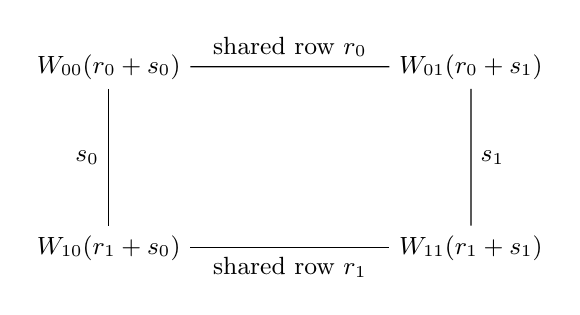
\begin{tikzpicture}[every node/.style={font=\small},scale=1.15]
\node (a) at (0,2) {$W_{00}(r_0+s_0)$};
\node (b) at (4,2) {$W_{01}(r_0+s_1)$};
\node (c) at (0,0) {$W_{10}(r_1+s_0)$};
\node (d) at (4,0) {$W_{11}(r_1+s_1)$};
\draw (a) -- node[above] {shared row $r_0$} (b);
\draw (c) -- node[below] {shared row $r_1$} (d);
\draw (a) -- node[left] {$s_0$} (c);
\draw (b) -- node[right] {$s_1$} (d);
\end{tikzpicture}

\caption{A square after fixing the slice background. The four rows
$r_0,r_1,s_0,s_1$ are independent, but their four sums satisfy one parity
relation. Fourier expansion therefore leaves one common frequency.
Different squares of a collision-free cube use disjoint rows.}
\label{fig:square}
\end{figure}


For four possibly different real slice functions $W_{ab}$, direct
Fourier expansion gives
\begin{equation}\label{eq:square-fourier}
 \E_{r_0,r_1,s_0,s_1}
       \prod_{a,b\in\{0,1\}}W_{ab}(r_a+s_b)
 =\sum_\alpha\prod_{a,b\in\{0,1\}}\widehat W_{ab}(\alpha).
\end{equation}
Indeed averaging $r_0,r_1$ forces the two frequencies in each row
of the square to agree, and averaging $s_0,s_1$ forces agreement
between these rows. Using the coefficient bound on two factors and
Cauchy--Schwarz and Parseval on the other two, the absolute value
of~\eqref{eq:square-fourier} is at most
\begin{equation}\label{eq:square-bound}
 \eps_0^2\sum_\alpha
       |\widehat W_{10}(\alpha)\widehat W_{11}(\alpha)|
 \le\eps_0^2H^2.
\end{equation}

Different squares use disjoint rows in both tables: any change in one
of the other $m-2$ coordinates changes a retained coordinate of
every such row. Conditional on the fixed background, their products
are consequently independent. Their slice functions may share that
background, which does not affect this independence. The absolute
conditional expectation of the full cube product is therefore at most
$(\eps_0^2H^2)^{2^{m-2}}$.
Combining this with the collision bound and
\eqref{eq:box-outer-average}, and using
$(a+b)^{1/Q}\le a^{1/Q}+b^{1/Q}$ for $a,b\ge0$, gives
\begin{equation}\label{eq:pair-correlation}
 \E\mathfrak d_Y(w^{ij})
 \le2A_0(m/\ell)^{1/2^m}
     +\sqrt{H(\gamma+H^2/A_0)}.
\end{equation}
The maximizing face signs were eliminated by the deterministic
inequality before the conditional independence argument was used.
No independence assumption about those signs is involved.

\subsection{Choosing parameters and completing inner decoding}
\label{sec:inner-completion}

For any two fields on a fixed box,
$|\mathfrak d_Y(u)-\mathfrak d_Y(v)|\le\E_{x\in Y}|u_x-v_x|$.
Thus~\eqref{eq:box-restriction}, localization, the processing losses,
and~\eqref{eq:pair-correlation} imply, for each pair class,
\begin{align}
 \E\mathfrak d_X(L^{ij})
 \le{}&\underbrace{\sigma^{-1}
       \sqrt{(s+Rm)\ell/(n-1)}}_{e_{\mathrm{loc}}}
       +\frac{\sigma^{-2}}H
       +\underbrace{\sigma^{-1}\sqrt{C_0/\gamma}
           (\theta^2+mpN/\sigma^2)^{1/4}}_{e_{\mathrm{atom}}}
       \notag\\
      &+\frac{\sigma^{-2}}{A_0}
       +2A_0(m/\ell)^{1/2^m}
       +\sqrt{H(\gamma+H^2/A_0)}.
 \label{eq:six-errors}
\end{align}
For class $0$, the corresponding bound is
\begin{equation}\label{eq:zero-errors}
 \E\mathfrak d_X(L^0)
 \le e_{\mathrm{loc}}+\frac{2\sigma^{-2}}{A_0}
      +2A_0(m/\ell)^{1/2^m}.
\end{equation}

\begin{proof}[Proof of Theorem~\ref{thm:inner}]
The smoothing parameters were fixed in
Proposition~\ref{prop:correlation}. Choose $m$ as in
\eqref{eq:choose-m}, define $d_0$ by~\eqref{eq:class-target}, and set
$e=d_0/10$. Make the following successive choices, each with strict
slack:
\begin{enumerate}[label=\arabic*.,leftmargin=*]
 \item Choose a positive integer $H$ with $\sigma^{-2}/H<e$.
 \item Choose a positive rational $\gamma$ with $H\gamma<e^2/4$.
 \item Choose a positive integer $A_0$ so large that
       $2\sigma^{-2}/A_0<e$ and $H^3/A_0<e^2/4$.
       These choices give
       $\sqrt{H(\gamma+H^2/A_0)}<e$.
 \item Choose an integer $\ell\ge2$ so large that
       $2A_0(m/\ell)^{1/2^m}<e$.
 \item Choose an integer $n>\ell$ so large that
       $\sigma^{-1}\sqrt{(s+Rm)\ell/(n-1)}<e$.
 \item Now $N=n^m$, $M=mn^{m-1}$ and
       $C_0=4^M\binom{N+s}{s}$ are fixed. Choose positive rationals
       $p,\theta<1$ so small that
       \[
        \theta^2+\frac{mpN}{\sigma^2}
        <\frac{e^4\sigma^4\gamma^2}{C_0^2}.
       \]
       This makes $e_{\mathrm{atom}}<e$.
\end{enumerate}
All choices are finite and use explicit inequalities. Roots in these
inequalities can be removed by raising positive quantities to integer
powers, so rational arithmetic and integer search suffice. Neither the
alphabet size nor the distribution of the proof index enters them.

If the row-atom assertion failed for these $p,\theta$, the preceding
argument would apply. Each pair-class correlation in
\eqref{eq:six-errors} would be less than $6e<d_0$, and the class-$0$
correlation in~\eqref{eq:zero-errors} would be less than $3e<d_0$.
Summing over the $1+\binom m2$ classes would give
\[
 \E\mathfrak d_X(L)<(1+\tbinom m2)d_0=\frac1{4T},
\]
contradicting~\eqref{eq:class-correlation-lower}. This proves the
claimed probability at least $p$ of an odd conditional coefficient
of magnitude at least $\theta$. The pointwise bound on $h_x$ is
\eqref{eq:gradient-bounds}, completing
Theorem~\ref{thm:inner}.
\end{proof}

\section{An outer game with affine hints}
\label{sec:outer}

This Section constructs the outer game and proves the two properties
used in Section~\ref{sec:composition}: soundness with shared affine hints,
and approximate joint uniformity of pulled-back affine functions.

Smooth equation--variable sampling and Fourier decoding have antecedents
in Khot and Safra~\cite[Sections~3.2--3.4 and~5.2]{KS13}.
Khot, Minzer and Safra~\cite[Sections~3.3--3.4]{KMS17} use shared linear
information and zero-advice coordinates; Dinur et al.~\cite[Section~5.2,
Lemma~5.4]{DKKMS2025} give a related shared-subspace formulation.
We prove both properties for the exact questions and hints defined below.

Let $\mathcal E=(E^{(1)},\ldots,E^{(M_0)})$ be the nonempty uniform
equation list supplied by Theorem~\ref{thm:max3lin}. An equation question
$E$ consists of its ordered three variable names $v(E,1),v(E,2),v(E,3)$
and its right-hand side $\tau_E\in\F_2$. Thus it asks that
\[
 x_{v(E,1)}+x_{v(E,2)}+x_{v(E,3)}=\tau_E.
\]
The list may have repeated equations, and variable names may repeat within
an equation. Sampling is uniform over list entries, but equal equation
questions have identical encodings: an index distinguishing equal list
entries is not part of a player's question.

\subsection{Questions, fresh slots, and canonical functions}

For an equation $E$, put
\[
 A(E)=\{a\in\F_2^3:
        a_1+a_2+a_3=\tau_E,\quad
        a_p=a_{p'}\text{ whenever }v(E,p)=v(E,p')\}.
\]
This is a nonempty affine space of dimension at most two. Indeed, after
identifying repeated variable names, there are $k\le3$ free bit slots and
one nonzero linear equation: at least one multiplicity is odd because the
sum of the multiplicities is three. The equation therefore has rank one,
and $\dim A(E)=k-1$.

Fix integers $t\ge t_0\ge1$. An \emph{outer sample} $e$ is drawn as follows.
First draw $t$ independent uniform list entries, with resulting equation
questions $E_1,\ldots,E_t$, and let
\[
 U=(E_1,\ldots,E_t),\qquad A_U=\prod_{j=1}^t A(E_j).
\]
Next draw a uniform $t_0$-element subset $H\subseteq[t]$. For each $j\in H$,
independently draw $p_j\in[3]$ uniformly. The second question is the ordered,
tagged tuple $V=(V_1,\ldots,V_t)$, where
\[
 V_j=\begin{cases}
       (\mathrm{variable},v(E_j,p_j)),&j\in H,\\
       (\mathrm{equation},E_j),&j\notin H.
     \end{cases}
\]
In particular, a variable question contains its variable name and the
coordinate $j$ in the ordered tuple, but neither its position $p_j$ nor
its originating equation. Set
\[
 A_V=\prod_{j=1}^t A_{V,j},\qquad
 A_{V,j}=\begin{cases}\F_2,&j\in H,\\\F_2^3,&j\notin H.\end{cases}
\]
Every displayed slot in this product is unrestricted. Even when the same
variable name occurs more than once, no equalities between these slots are
imposed. Likewise, the slots belonging to distinct coordinates of $A_U$
are separate; its only equalities between repeated names are those inside
a single factor $A(E_j)$. These fresh slots are essential both to independent
repetition and to the distribution of affine forms below.

Define the affine map $\pi_e:A_U\to A_V$ coordinatewise by
\begin{equation}\label{eq:outer-projection}
 (\pi_e(a))_j=\begin{cases}(a_j)_{p_j},&j\in H,\\a_j,&j\notin H.\end{cases}
\end{equation}
The verifier accepts labels $a\in A_U$ and $b\in A_V$ precisely when
$\pi_e(a)=b$. The map need not be onto: the unrestricted full triples on
the second side need not satisfy their equations. Pullback is the linear
map
\[
 \pi_e^*:D(A_V)\longrightarrow D(A_U),\qquad L\longmapsto L\circ\pi_e,
\]
and preserves the constant-one function.

We specify exactly what a question and an affine hint reveal. Every actual
$U$ or $V$ is the tuple just defined, without extra information identifying
its occurrence in $e$. Put its alphabet in lexicographic order as a subset
of its displayed bit slots. A function on that alphabet is represented by
its complete truth table in this order. In particular, a hint in $D(A_U)$
or $D(A_V)$ is the function itself, with this canonical encoding. It is not
accompanied by a formula, its original coefficients on another alphabet,
or an encoding of the map through which it was pulled back. Equal functions
on the same actual question have equal encodings. The same convention will
apply to Boolean queries in the bit proofs. Thus a response function at a
given question cannot distinguish different descriptions of the same query.

For an integer $q\ge0$, the \emph{game with $q$ affine hints} additionally
draws independent uniform functions $L_1,\ldots,L_q\in D(A_V)$. The first
player receives
\[
 (U,\pi_e^*L_1,\ldots,\pi_e^*L_q)
\]
and the second receives $(V,L_1,\ldots,L_q)$. The acceptance condition is
still $\pi_e(a)=b$. Giving independent shared or private randomness to these
players does not change the upper bounds on its value.

\subsection{Soundness despite the affine hints}

Consider first the ordinary equation-versus-variable game: draw a uniform
list entry $E$, choose a uniform position $p\in[3]$, give $E$ to the first
player and only $v(E,p)$ to the second, and ask for $a\in A(E)$ and a bit
$b$. Accept when $a_p=b$. Equivalently the first answer alphabet can be
$\F_2^3$ with invalid answers rejected, so the answer sizes are at most
eight and two.

\begin{lemma}\label{lem:base-equation-game}
If no assignment satisfies more than $3/4$ of the equation list, the
ordinary equation-versus-variable game has value at most $11/12$.
Consequently its ordinary $r$-fold repetition has value at most $c^r$, for
the effective universal constant $c<1$ of
Theorem~\ref{thm:parallel-repetition}, for every $r\ge0$.
\end{lemma}
\begin{proof}
Fix a deterministic second strategy. Its bit for each variable name defines
a global assignment. On at least $1/4$ of the sampled equations this
assignment violates the equation. Every valid first answer to one of these
equations disagrees with this assignment in at least one of the three
positions, so a uniform position detects disagreement with probability at
least $1/3$. An invalid answer is rejected in every position. The overall
failure probability is therefore at least $1/12$. Repeated variable names
do not affect the argument: equality at all three positions would still
give precisely the violated assignment on that equation. The repeated
bound follows from Theorem~\ref{thm:parallel-repetition}; its hypotheses
depend only on this value bound and the two answer sizes.
\end{proof}

\begin{lemma}[Hint soundness]\label{lem:hint-soundness}
Suppose no assignment satisfies more than $3/4$ of the equation list. For
every $q\ge0$ and $t\ge t_0\ge1$, the value of the game with $q$ affine
hints is at most
\begin{equation}\label{eq:hint-bound}
 \bigl(1-2^{-q}(1-c)\bigr)^{t_0}.
\end{equation}
The bound also applies to strategies using arbitrary independent shared
or private randomness. In particular, for fixed $q$ and any prescribed
rational $s>0$, an effective choice of $t_0$ makes the bound strictly less
than $s$, simultaneously for every $t\ge t_0$, every equation-list size,
and every completeness parameter in Theorem~\ref{thm:max3lin}.
\end{lemma}
\begin{proof}
Use the unrestricted slots of $A_V$ to generate the hints. Let $z_j$ denote
the one-bit coordinate when $j\in H$, and let $z_{jp}$, $p\in[3]$, denote
the three coordinates when $j\notin H$. A uniform affine form has the
unique expression
\begin{equation}\label{eq:hint-coefficients}
 L_\ell(z)=\kappa_\ell+
       \sum_{j\in H}\beta_{\ell j}z_j+
       \sum_{j\notin H}\sum_{p=1}^3\beta_{\ell jp}z_{jp}.
\end{equation}
All coefficients and constants in these expressions, for $1\le\ell\le q$,
are independent uniform bits. They can be sampled after $H$ and before
any equation or position, because the abstract slots in this expression
depend only on $H$. Thus their distribution is independent of all sampled
equations and positions.

Define the active coordinates by
\[
 A=\{j\in H:\beta_{\ell j}=0\text{ for every }1\le\ell\le q\}.
\]
For each $j\in H$ its vector of $q$ coefficients is uniform in $\F_2^q$,
independently across $j$. Consequently
\begin{equation}\label{eq:active-binomial}
 |A|\sim\operatorname{Bin}(t_0,2^{-q}).
\end{equation}
Conditional on $H$, the active set and the coefficient bits are independent
of the equation and position samples. The equations are also independent
of $H$. When $q=0$, all hidden coordinates are active and
\eqref{eq:active-binomial} means $|A|=t_0$ deterministically.

For the analysis give both players the following additional information:
$H$, every coefficient and constant in \eqref{eq:hint-coefficients}, and
all equation samples and all chosen positions outside $A$. Denote this
background by $W$. It determines $A$ without inspecting its equation or
position samples. Conditional on any possible $W$, the pairs
\[
 (E_j,p_j),\qquad j\in A,
\]
are still independent samples of a uniform equation-list entry and an
independent uniform position in $[3]$. This follows directly from the
product sampling distribution: once $H$ and the coefficients are fixed,
$A$ is fixed, and conditioning on samples in its complement does not
change the samples in $A$.

We now show that, for fixed $W$, ordinary repeated-game questions in the
active coordinates simulate each player's original information exactly.
List $A$ in increasing order, so that its $|A|$ coordinates can be identified
with an ordinary repetition.
\begin{enumerate}[label=\textup{(\roman*)}]
\item The first player receives the active equation questions $(E_j)_{j\in A}$.
Together with $W$, these reconstruct all of $U$ and hence $A_U$.
For every hint the active summands in \eqref{eq:hint-coefficients} are
identically zero. On any $a\in A_U$, therefore,
\[
 (\pi_e^*L_\ell)(a)=\kappa_\ell+
    \sum_{j\in H\setminus A}\beta_{\ell j}(a_j)_{p_j}+
    \sum_{j\notin H}\sum_{p=1}^3\beta_{\ell jp}(a_j)_p.
\]
Every position appearing on the right is in the background. Thus the first
player can compute the canonical truth table of each pulled-back hint,
without receiving any active $p_j$ or active variable question from the
second side. Although the domain $A_U$ depends on active equations, these
are exactly the first player's own repeated-game questions.
\item The second player receives only the active variable names
$(v(E_j,p_j))_{j\in A}$. Together with $W$ and the tags specified by $H$,
these reconstruct $V$ and $A_V$. Formula~\eqref{eq:hint-coefficients}, whose
active coefficients vanish, computes every direct hint on this alphabet.
Thus the second player can compute its canonical truth table without
receiving an active equation or the chosen position within one.
\end{enumerate}
These reconstructions also explain why the representation of a hint
matters. No metadata attached to a zero summand is present in the actual
message. Restricting the zero function to an affine domain cannot create
an offset or convey a hidden position. All nonzero contributions and their
possible affine offsets are determined by the background and the receiving
player's own question.

Apply the original response functions to the reconstructed information,
and restrict their answers to the active coordinates. This defines a
strategy for the ordinary $|A|$-fold repeated game, with $W$ fixed as a
parameter. Acceptance of the full outer sample implies acceptance in
every active coordinate, since \eqref{eq:outer-projection} imposes exactly
the ordinary equation-versus-variable comparison there. By
Lemma~\ref{lem:base-equation-game}, its conditional probability is at most
$c^{|A|}$; for $A=\varnothing$ this is the trivial bound one.

This reasoning includes coincidences between variable names or equation
questions in different coordinates, and coincidences with the exposed
background. Independent samples may coincide without ceasing to have a
product distribution. Once $W$ is fixed, the simulated strategies may use
all information about such coincidences obtainable from their respective
questions, just as arbitrary strategies for ordinary repetition may do.
No equality between fresh answer slots, nor any further information about
an active question on the opposite side, has been supplied.

Average over $W$ and use \eqref{eq:active-binomial}. The binomial generating
function gives
\[
 \Prob[\text{outer acceptance}]
 \le\E c^{|A|}
 =\sum_{r=0}^{t_0}\binom{t_0}{r}(2^{-q}c)^r
                       (1-2^{-q})^{t_0-r}
 =\bigl(1-2^{-q}(1-c)\bigr)^{t_0}.
\]
One may first fix all independent random seeds of the players, apply the
bound, and then average; this covers the stated random strategies.

Finally replace $c$, if necessary, by an effectively chosen rational
number $\bar c$ with $c\le\bar c<1$. Successively multiplying the rational
number $1-2^{-q}(1-\bar c)<1$ finds an integer $t_0$ whose power is strictly
less than $s$. This finite procedure is independent of $t$, the instance,
and its completeness error. It supplies the asserted effective choice.
\end{proof}

\subsection{Joint marginal smoothness}

The following estimate concerns the joint distribution of several forms
pulled back through the same outer sample. Conditioning is on $U$ only;
in particular it is not conditioning on any previously received hint.
For finite probability distributions $\mu,\nu$, use
$\TV(\mu,\nu)=\frac12\sum_x\abs{\mu(x)-\nu(x)}$.

\begin{lemma}[Joint smoothness]\label{lem:smoothness}
Fix any actual first question $U$, integers $d\ge1$ and $t\ge t_0\ge1$,
and draw the remaining outer sample conditional on $U$. Draw
$L_1,\ldots,L_d$ independently and uniformly from $D(A_V)$. Then
\begin{equation}\label{eq:smoothness-bound}
 \TV\left(\mathcal L\bigl((\pi_e^*L_1,\ldots,\pi_e^*L_d)\mid U\bigr),
                 \operatorname{Unif}(D(A_U)^d)\right)
 \le\frac12\sqrt{(2^{4dt_0}-1)\frac{t_0^2}{t}}.
\end{equation}
The bound is uniform in $U$ and the equation list, including repeated
variable names and zero-dimensional local alphabets. For fixed $d,t_0$
and positive rational $\Delta$, an effective integer $t\ge t_0$ makes
the right-hand side strictly less than $\Delta$.
\end{lemma}
\begin{proof}
Write $A_j=A(E_j)$ and $r_j=\dim A_j\le2$. Choose, using $E_j$ alone,
an affine origin $o_j\in A_j$ and an injective linear map
$T_j:\F_2^{r_j}\to\F_2^3$ with image the translation space of $A_j$.
Thus every label has a unique expression
\[
 a_j=o_j+T_ju_j,\qquad u_j\in\F_2^{r_j}.
\]
For example, lexicographic search and binary Gaussian elimination make
these choices canonical and effective. In these product coordinates a
form on $A_U$ consists of one constant bit and a linear part in each
coordinate group $\F_2^{r_j}$. A $d$-tuple of forms consequently consists
of $d$ constant bits and groups
\[
 \xi_j\in(\F_2^{r_j})^d,\qquad 1\le j\le t.
\]

Generate the $d$ forms by their independent raw coefficients and constants
on the unrestricted slots of $A_V$, as in
\eqref{eq:hint-coefficients}. After pullback, their constant bits are the
original independent uniform constants plus offsets determined by the
other coefficients, the positions, and the origins $o_j$. Conditional
on all those other data, this addition is a translation of $\F_2^d$.
Hence the resulting constants are jointly uniform and independent of
every linear part, of $H$, and of the chosen positions. Their common
uniform factor contributes no total-variation distance, so it suffices
to analyze the joint linear parts $(\xi_1,\ldots,\xi_t)$.

Fix $H$. If $j\notin H$, a single form has independent uniform coefficient
vector $w\in\F_2^3$ on its three raw slots; its pulled-back linear part
is $T_j^{\mathsf T}w$. The map $T_j^{\mathsf T}$ has rank $r_j$ and is
onto $\F_2^{r_j}$. Every fiber therefore has the same size, so its output
is uniform. All $d$ forms in this group are independent, and their joint
law is the uniform law $\mu_j$ on $(\F_2^{r_j})^d$.

If $j\in H$, condition first on its chosen position $p_j$. The $\ell$th
form has a uniform bit coefficient $\beta_{\ell j}$ on that slot, so its
linear part is $\beta_{\ell j}v_{j,p_j}$, where $v_{j,p}$ is the linear
part of the $p$th coordinate of $o_j+T_ju_j$. Average over the single
uniform choice of $p_j$ shared by all $d$ forms, to obtain a distribution
$Q_j$ on $(\F_2^{r_j})^d$. Its density $\rho_j$ with respect to $\mu_j$
satisfies
\begin{equation}\label{eq:local-density}
 \E_{\mu_j}\rho_j=1,\qquad
 0\le\rho_j\le2^{r_jd}\le2^{2d}.
\end{equation}
Indeed, every point of this finite space has uniform mass $2^{-r_jd}$,
whereas its $Q_j$ mass is at most one. This argument allows a position's
linear part to be zero or to coincide with another position's linear
part. If $r_j=0$, the space is a singleton and $\rho_j=1$.

For fixed $H$, the linear-part groups are independent across $j$:
their coefficients are independent, and the positions in distinct hidden
coordinates are independently sampled. Fresh slots give this independence
even when variable names in different equations coincide. Relative to
the product uniform measure $\mu=\prod_{j=1}^t\mu_j$, their joint density
is therefore
\[
 g_H(\xi_1,\ldots,\xi_t)=\prod_{j\in H}\rho_j(\xi_j).
\]
The densities $\rho_j$ depend on $U,d,j$ but not on the other elements
of $H$. Since $H$ is uniform and independent of $U$, the desired mixed
density is $g=\E_H g_H$.

Let $H'$ be an independent uniform $t_0$-element subset of $[t]$.
If $H\cap H'=\varnothing$, independence of the coordinate groups and
\eqref{eq:local-density} give
$\E_\mu g_Hg_{H'}=1$. For every $H,H'$, the pointwise bound
$g_Hg_{H'}\le2^{4dt_0}$ gives the sufficient bound
$\E_\mu g_Hg_{H'}\le2^{4dt_0}$. Moreover, for fixed $H$,
\[
 \Prob[H\cap H'\ne\varnothing]
 \le\sum_{j\in H}\Prob[j\in H']
 =\frac{t_0^2}{t}.
\]
Since $\E_\mu g=1$, it follows that
\begin{align*}
 \E_\mu(g-1)^2
 &=\E_{H,H'}\E_\mu g_Hg_{H'}-1\\
 &\le(2^{4dt_0}-1)\Prob[H\cap H'\ne\varnothing]\\
 &\le(2^{4dt_0}-1)\frac{t_0^2}{t}.
\end{align*}
Cauchy--Schwarz now yields
$\TV(g\mu,\mu)=\frac12\E_\mu\abs{g-1}
\le\frac12\sqrt{\E_\mu(g-1)^2}$, proving
\eqref{eq:smoothness-bound}, including the independent uniform constants.

All estimates used only $r_j\le2$, so the bound is uniform as asserted.
For effectiveness, it is enough to choose an integer
\[
 t\ge t_0,\qquad
 t>\frac{(2^{4dt_0}-1)t_0^2}{4\Delta^2}.
\]
The right-hand side is an explicitly computable rational number for fixed
$d,t_0,\Delta$. No parameter depending on $U$ occurs in this choice.
\end{proof}

\begin{remark}\label{rem:joint-smoothness-use}
Because \eqref{eq:smoothness-bound} is uniform in $U$, it may be averaged
over any distribution of $U$ and any extra randomness independent of the
outer sample. In particular, if a bounded statistic is chosen as a function
of $U$ and some of the pulled-back forms, one may apply Lemma~\ref{lem:smoothness} to the
joint collection of all forms used by that statistic. For a statistic
bounded in absolute value by $B$, the change in expectation is at most
$2B$ times the displayed total-variation bound. This does not assert
uniformity of one form conditional on previously revealed forms.
\end{remark}

Finally, these outer games are explicit finite objects. Their complete
sampling space has
\[
 M_0^t\binom{t}{t_0}3^{t_0}
\]
equally likely draws, counting repeated list entries with their
multiplicities. There are at most $2^{2t}$ labels at a first question and
$2^{3t-2t_0}$ labels at a second question. Their affine spaces, functions,
canonical truth tables, and projections are all enumerable by binary
linear algebra and finite evaluation. For fixed $t,t_0,q,d$ these local
enumerations have constant size independent of the input. Comparing
actual question encodings and identifying equal ones takes polynomial
bit complexity. Thus the fresh-slot and canonical-function conventions
introduce no oracle or uncharged lookup table.

\section{Composition and soundness of the bit comparisons}
\label{sec:composition}

We now compose the inner test with the outer game. The main issue is that the
first player's Fourier truncation depends on the shared background. The joint
form of Lemma~\ref{lem:smoothness} is designed to retain that dependence.

\begin{proposition}[A gap for bit comparisons]\label{prop:bit-gap}
For every fixed integer $J\ge20$, effective choices of constants give a
four-test comparison system with the following properties. It is constructed
from the uniform equation list in Theorem~\ref{thm:max3lin}, for a fixed
completeness error $\zeta>0$ chosen by the construction. Every test compares
two bits in folded proof tables, and its contribution to cost is its failure
probability divided by a positive rational budget $b_j$.
In the YES case there are proof tables of cost at most $4$; in the NO case
every collection of proof tables has cost greater than $J$.
Alphabet sizes are bounded by effective constants depending only on $J$,
and all local numerical parameters depend only on $J$.
\end{proposition}

\begin{proof}
Apply Theorem~\ref{thm:inner} with $J$, taking its atom constants $p,\theta$
to be positive rationals by decreasing them if necessary. Set
\[
 M=mn^{m-1},\qquad q=M-1,\qquad M_*=\frac{\sqrt N}{\sigma}.
\]
The counts $t_0\le t$ of the outer game will be chosen below. Give each actual
first question $U$ a folded bit proof $f_U$ on $A_U$, and each actual second
question $V$ a folded bit proof $f_V$ on $A_V$. The same question always uses
the same proof; an occurrence of a hidden variable is never separately
indexed by its unrevealed equation or position.

The first three tests are those of Theorem~\ref{thm:inner}, applied to $f_V$
under the marginal distribution of $V$. For the fourth test sample a full
outer edge $e$, an independent uniform face array $B$ over $D(A_V)$, and the
Gaussian query table $P=P_{c+\sigma g,\eta\lambda}$ on the common code $\C$.
Compare
\begin{equation}\label{eq:fourth-test}
 f_U\bigl(P(\pi_e^*B)\bigr)
 \quad\hbox{and}\quad
 f_V\bigl(P(B)\bigr).
\end{equation}
Here $\pi_e^*$ acts on every entry of $B$. The Gaussian table on $\C$ is
literally the same on both sides, even if distinct codewords have identical
pullbacks at one alphabet. Let $b_4>0$ be a small rational budget, to be fixed
shortly, and define
\[
 \Cost(f)=\sum_{j=1}^4\frac{\Prob[\text{test $j$ fails}]}{b_j}.
\]

Suppose, toward a contradiction in the NO case, that $\Cost(f)\le J$.
Each of the first three failure bounds required by Theorem~\ref{thm:inner}
then holds, including the random index $V$. Draw an outer edge $e$, a uniform
$i\in[m]$ and $x\in X$, and independent $c$. The $q$ rows other than
$B^i_{x_{-i}}$ will serve as the independent uniform background forms allowed
in Lemma~\ref{lem:hint-soundness}. Put them in a fixed order depending only on
the public $i,x$. The two players receive these rows on their own alphabets,
and use $c,i,x$ as additional public randomness, independent of the game.
From their respective information they form the one-row functions
\begin{align}
 H_V(b)&=h_{x,V}\bigl(B[B^i_{x_{-i}}\leftarrow b],c\bigr),
      &&b\in D(A_V),\label{eq:HV}\\
 H_U(a')&=h_{x,U}\bigl((\pi_e^*B)
                 [B^i_{x_{-i}}\leftarrow a'],c\bigr),
      &&a'\in D(A_U).\label{eq:HU}
\end{align}
The notation in \eqref{eq:HU} simply means filling the missing entry of the
received array with a free argument. The first player needs no knowledge of
$e$ or $V$ to define $H_U$. Both functions are bounded in absolute value by
$M_*$.

\paragraph{The two row functions are close.}
For fixed $e,B,c$, apply \eqref{eq:gaussian-derivative} to the difference
between the two bits in \eqref{eq:fourth-test}, using the same $g,\lambda$.
Bessel's inequality for the orthonormal functions $g_x$ gives
\[
 \frac1N\sum_x
 \abs{h_{x,V}(B,c)-h_{x,U}(\pi_e^*B,c)}^2
 \le\frac1{\sigma^2}\E_{g,\lambda}
 \abs{f_V(P(B))-f_U(P(\pi_e^*B))}^2.
\]
Averaging $e,B,c$ bounds the right-hand side by $4Jb_4/\sigma^2$.
Integrating the missing row in \eqref{eq:HV} restores a fully independent
uniform array $B$, regardless of $i,x$. Thus
\begin{equation}\label{eq:row-comparison}
 \E\norm{H_V-H_U\circ\pi_e^*}_{L^2(D(A_V))}^2
 \le\frac{4Jb_4}{\sigma^2}.
\end{equation}
Choose a positive rational $b_4$ so small that
\begin{equation}\label{eq:budget-choice}
 \frac{64Jb_4}{\sigma^2\theta^2}<\frac p4.
\end{equation}
Markov's inequality then makes the norm in \eqref{eq:row-comparison} less
than $\theta/4$, except on an event of probability less than $p/4$.

\paragraph{Diffuse first-side frequencies remain small after pullback.}
Choose a positive rational $u<1$. At each first-player information state,
let $r_U$ be $H_U$ with all Fourier terms of magnitude at least $u$ removed.
Parseval and the bound $\abs{H_U}\le M_*$ give
\begin{equation}\label{eq:remainder-bounds}
 \#\{\alpha:\abs{\widehat H_U(\alpha)}\ge u\}
 \le\frac{M_*^2}{u^2},\qquad
 \sum_\alpha\abs{\widehat r_U(\alpha)}^4\le u^2M_*^2,
 \qquad
 \norm{r_U}_\infty\le M_r:=M_*+\frac{M_*^2}{u}.
\end{equation}
For the last bound, each removed coefficient satisfies
$\abs{a}\le\abs{a}^2/u$.

We claim that if the total-variation bound of Lemma~\ref{lem:smoothness} for
$d=q+3$ is at most $\Delta$, then
\begin{equation}\label{eq:restricted-fourth}
 \E\sum_{\beta\in D(A_V)^*}
       \abs{\widehat{r_U\circ\pi_e^*}(\beta)}^4
 \le u^2M_*^2+2\Delta M_r^4.
\end{equation}
To prove this, fix $U$ and the independent public randomness $c,i,x$.
For fixed background and $e$, identity \eqref{eq:fourth-moment} expresses the
Fourier sum on the left as the average of
\[
 r_U(\pi_e^*a)r_U(\pi_e^*b)r_U(\pi_e^*c')
 r_U\bigl(\pi_e^*(a+b+c')\bigr),
\]
where $a,b,c'$ are independent uniform forms on $A_V$. Pullback is linear
on the spaces of affine forms, so its fourth argument is determined by the
first three. The entire expression, including the choice of $r_U$, depends
only on $U,c,i,x$ and the $q+3$ pulled-back forms consisting of the background
and these three additional arguments. It is bounded by $M_r^4$ in absolute
value. Replace their joint distribution by independent uniform forms on
$A_U$. Lemma~\ref{lem:smoothness} changes the expectation by at most
$2\Delta M_r^4$. Under the replacement, conditioning on the background fixes
$r_U$, and \eqref{eq:fourth-moment} and \eqref{eq:remainder-bounds} bound its
expectation by $u^2M_*^2$. Averaging proves
\eqref{eq:restricted-fourth}. This argument uses joint total variation; it
does not conditionally replace the missing row while keeping a nonuniform
background fixed.

First choose $u>0$ rational sufficiently small, and then require a sufficiently
small positive rational $\Delta$, so that
\begin{equation}\label{eq:remainder-choice}
 \frac{256\bigl(u^2M_*^2+2\Delta M_r^4\bigr)}{\theta^4}<\frac p4.
\end{equation}
By \eqref{eq:restricted-fourth} and Markov's inequality, no Fourier
coefficient of $r_U\circ\pi_e^*$ has magnitude at least $\theta/4$, except
on an event of probability less than $p/4$.

\paragraph{Local lists give a strategy for the outer game.}
Theorem~\ref{thm:inner} supplies an odd coefficient $\beta$ of $H_V$ with
magnitude at least $\theta$ with probability at least $p$. Combining that
event with the two preceding estimates leaves probability at least $p/2$.
On this event, the coefficient of $H_U\circ\pi_e^*$ at $\beta$ has magnitude
greater than $3\theta/4$, since every coefficient is bounded by the $L^2$
norm of a function. The coefficient of its remainder has magnitude less
than $\theta/4$. Consequently the pullback of the removed part has a nonzero
coefficient at $\beta$. At least one removed frequency $\alpha$ therefore
satisfies
\[
 (\pi_e^*)^*\alpha=\beta.
\]
This conclusion permits multiple frequencies to have the same image:
a nonzero sum has at least one nonzero summand. Since $\pi_e^*(1)=1$ and
$\beta$ is odd, such an $\alpha$ is odd as well.

The first player lists the odd frequencies of $H_U$ of magnitude at least
$u$, and the second lists the odd frequencies of $H_V$ of magnitude at least
$\theta$. These lists are functions of their own information. By
Lemma~\ref{lem:odd-labels}, they are lists of labels, and on the event just
described they contain a pair agreeing under $\pi_e$. Their sizes are at
most $M_*^2/u^2$ and $M_*^2/\theta^2$. Choose uniformly from nonempty lists
and choose any fixed label when a list is empty. With independent private
randomness, the resulting strategy succeeds with probability at least
\begin{equation}\label{eq:decoder-success}
 s_*:=\frac{p/2}{(1+M_*^2/u^2)(1+M_*^2/\theta^2)}>0.
\end{equation}
The strategy is used only to bound the value of a finite game. Its Fourier
computations need not be efficient, and its independent continuous public
randomness does not raise the game value above the maximum deterministic
value.

\paragraph{Parameter order and contradiction.}
All quantities so far depend only on the inner constants and $J$.
Choose $t_0$ effectively so that the upper bound in
Lemma~\ref{lem:hint-soundness} is strictly below $s_*$ for the fixed $q$.
Then choose $t\ge t_0$ so large that Lemma~\ref{lem:smoothness} gives the
required $\Delta$ for $d=q+3$. Equation \eqref{eq:decoder-success}
contradicts the hinted-game upper bound, proving that no NO-case proof has
cost at most $J$.

Finally choose a positive rational $\zeta$ with $t\zeta\le b_4$ and invoke
Theorem~\ref{thm:max3lin}. Its NO bound is always $3/4$, independently of
$\zeta$, so this last choice does not affect the repetition constants.
In the YES case let a global assignment satisfy at least $1-\zeta$ of the
equations. Give each $V$ its values at all requested slots. Give $U$ these
values whenever all its equations are satisfied, and choose any label in
$A_U$ otherwise. The first labels lie in their required affine alphabets,
and the labels agree under $\pi_e$ except on an event of probability at most
$t\zeta$. Use evaluation proofs at these labels. Lemma~\ref{lem:honest}
bounds each of the first three normalized costs by one; agreement of labels
makes the fourth comparison exact, so its normalized cost is also at most
one. This proves the YES bound.

The order of choices is, explicitly,
\[
 J\ \longrightarrow\ \text{inner constants}
 \longrightarrow\ b_4,u,\Delta,s_*
 \longrightarrow\ t_0\ \longrightarrow\ t\ \longrightarrow\zeta.
\]
All strict inequalities can be imposed with rational slack and integer
searches using the displayed bounds. In these searches $M_*^2=N/\sigma^2$
is rational; the possibly irrational quantity $M_r$ may be bounded above
by the rational number $N/\sigma+N/(\sigma^2u)$ before choosing $\Delta$. The complete construction therefore
has effective constants independent of the input length.
\end{proof}

\section{A deterministic finite reduction to simple graphs}
\label{sec:finite}

Fix an integer $K\ge2$, put $J=10K$, and make the effective parameter
choices in Proposition~\ref{prop:bit-gap}. Write $\Cost_\infty$ for its
cost, and put
\[
 W=\sum_{j=1}^4 b_j^{-1}.
\]
This is a positive rational constant depending only on $K$. The Gaussian
randomness will now be replaced by one finite rational distribution. We
retain the full joint distribution of the queried sign tables.

\subsection{Rational Gaussian sign tables}

Let $c,g\in\R^X$ and $\lambda\in\R^{\C}$ have independent standard
Gaussian coordinates. Define the two tables on $\C$
\begin{align*}
 T_0(z)&=\sgn\left(N^{-1/2}\sum_{x\in X}c_x(-1)^{z_x}\right),\\
 T_1(z)&=\sgn\left(N^{-1/2}\sum_{x\in X}(c_x+\sigma g_x)(-1)^{z_x}
                         +\eta\lambda_z\right).
\end{align*}
Their pair is a random element of a finite set of size
$2^{2|\C|}$. All four tests are deterministic functions of this pair and
their finite random choices. The first uses both tables. The second uses
the same $T_1$ for $B$ and $B'$. The third forces one entry of $T_1$ to the
two specified values. The fourth uses the same $T_1$ on the two outer
alphabets. Thus a single approximation of $(T_0,T_1)$ suffices.

\begin{lemma}[Effective finite comparisons]\label{lem:finite-game}
There is a deterministic construction, with all preliminary work depending
only on $K$, of a finite rational replacement for the four tests such that
\begin{equation}\label{eq:uniform-finite-error}
 \abs{\Cost_{\mathrm{fin}}(f)-\Cost_\infty(f)}<\frac12
 \qquad\text{for every collection of folded proof tables }f.
\end{equation}
Consequently its minimum cost is less than $9/2$ in the YES case, and every
proof has cost greater than $10K-1/2$ in the NO case. The rational
distribution replacing $(T_0,T_1)$ has a positive integer common
denominator depending only on $K$, computed by the construction.
\end{lemma}

\begin{proof}
We give a deterministic rational approximation with any prescribed rational
accuracy $0<\eps<1/4$. Set
\[
 d=2N+|\C|,\qquad S=2|\C|,\qquad A=2N+1.
\]
The $S$ unforced threshold inputs are linear forms in a vector
$Z\in\R^d$ of independent standard Gaussians. Each input for $T_0$ has
variance $1$, and each input for $T_1$ has variance
$1+\sigma^2+\eta^2$. Its coefficient vector has $\ell^1$ norm at most
\[
 (1+\sigma)\sqrt N+\eta\le A.
\]
These bounds do not require nonsingularity of the joint distribution of
the threshold inputs.

Choose an integer $T_G\ge1$ such that
\[
 d/T_G^2<\eps/4.
\]
The probability $\alpha$ that $Z\notin[-T_G,T_G]^d$ is at most $d/T_G^2$,
by the second-moment bound in each coordinate and a union bound. Partition
$[-T_G,T_G]$ into $L$ equal intervals of length $h=2T_G/L$, with rational
midpoints. Choose the integer $L$ large enough that
\begin{equation}\label{eq:gaussian-mesh-choice}
 SAh<\eps/4.
\end{equation}
Endpoint conventions for the intervals are immaterial to their Gaussian
masses. Rounding an interior vector to its cell midpoint changes any
threshold input by at most $Ah/2$. If the corresponding signs change,
the original threshold input has absolute value at most $Ah/2$.
A centered Gaussian of variance at least one has density at most one,
so the probability of this event for any one threshold is at most $Ah$.
The union bound over all $S$ thresholds is therefore at most $SAh$.
In particular, all unrounded ties have probability zero.

For completeness, this estimate can be combined with truncation without
losing control at the boundary. Couple $Z$ with a vector $Y$ as follows:
keep $Y=Z$ when $Z$ is in the cube, and otherwise draw $Y$ independently
from the Gaussian conditioned on the cube. Then $Y$ has exactly that
conditional law. On the event that $Z$ is outside, charge the full
probability $\alpha$; on its complement use the preceding sign-change
estimate. Hence the law of the original joint sign table and the law
obtained by rounding the conditioned Gaussian differ in total variation
by at most
\begin{equation}\label{eq:tail-and-grid-error}
 d/T_G^2+SAh<\eps/2.
\end{equation}

We next compute rational approximations to the conditioned Gaussian cell
masses, including their exact normalization. This step uses no real-number
oracle. Put $U=T_G^2/2$, and choose an integer $r\ge0$ such that
\[
 e_r:=\frac{U^{2r+1}}{(2r+1)!}
 \quad\text{satisfies}\quad 2dT_G e_r<\eps/4.
\]
This is a terminating search with rational comparisons. Indeed
$e_{r+1}/e_r=U^2/((2r+2)(2r+3))$, so after an effectively found index
the ratio is at most $1/2$. Define the rational polynomial
\[
 Q_r(v)=\sum_{j=0}^{2r}\frac{(-1)^jv^{2j}}{2^j j!}.
\]
Taylor's remainder for $e^{-u}$, with $u=v^2/2\ge0$, gives
\begin{equation}\label{eq:positive-density-polynomial}
 0\le Q_r(v)-e^{-v^2/2}\le e_r
 \qquad (|v|\le T_G).
\end{equation}
In particular $Q_r$ is strictly positive on the interval. For each grid
interval $I=[a,b]$, compute the rational number
\begin{equation}\label{eq:rational-cell-mass}
 w_I=\frac{\displaystyle\int_a^b Q_r(v)\dd v}
            {\displaystyle\int_{-T_G}^{T_G} Q_r(v)\dd v}.
\end{equation}
Both integrals are evaluated by the rational antiderivative
\[
 \sum_{j=0}^{2r}\frac{(-1)^jv^{2j+1}}{2^j j!(2j+1)}.
\]
Thus the $w_I$ are positive rationals and their sum is exactly one.

Here is a quantitative error bound for these cell masses. Write
$g(v)=e^{-v^2/2}$ on $[-T_G,T_G]$, let $Z_g=\int_{-T_G}^{T_G}g$, and let
$E_r=\int_{-T_G}^{T_G}(Q_r-g)$. Since $T_G\ge1$ and $e^{-u}\ge1-u$ for
$u\ge0$,
\[
 Z_g\ge\int_{-1}^1(1-v^2/2)\dd v>1,
 \qquad 0\le E_r\le2T_G e_r.
\]
The probability density $Q_r/(Z_g+E_r)$ is a mixture of $g/Z_g$ and
the normalized nonnegative residual $Q_r-g$, with residual mixture
weight $E_r/(Z_g+E_r)$ (if $E_r=0$ the densities coincide).
Their total variation distance is therefore at most $2T_G e_r$.
The Gaussian conditioned on the cube is a product of these
one-dimensional conditioned laws. Taking products increases the total
variation error by at most the sum of the coordinate errors, as follows
by replacing the coordinates one at a time. Rounding to the grid cannot
increase total variation. Consequently the grid distribution assigning
mass $\prod_{i=1}^d w_{I_i}$ to a cell has total variation distance at
most $2dT_G e_r<\eps/4$ from the rounded conditional Gaussian law.
Together with \eqref{eq:tail-and-grid-error}, this proves error less than
$\eps$ for the complete joint sign table.

Every sign at a rational midpoint is also computed exactly. A $T_0$
input has the sign of a rational number. Multiplying a $T_1$ input by
$\sqrt N>0$ expresses it as
\[
 a+b\sqrt N\qquad(a,b\in\mathbb Q).
\]
If $a,b$ have the same sign, or one is zero, its sign is immediate.
If their signs are opposite, compare the rationals $a^2$ and $Nb^2$;
the term of larger magnitude determines the sign, and equality is
an exact zero. Declare the sign of zero to be $+1$. This also handles
square $N$. Thus grid ties and all algebraic comparisons use finite
rational arithmetic.

Choose a common denominator $Q_1$ for the finitely many rationals $w_I$,
for example the product of their reduced positive denominators, and put
$Q=Q_1^d$. Every cell probability is an integer multiple of $1/Q$.
Enumerate the $L^d$ cells, compute their complete sign-table pairs, and
add the integer numerators for cells giving the same pair. This gives
an explicit rational law $\widehat\mu$ for $(T_0,T_1)$ with denominator
$Q$. The code $\C$, the grid, the polynomial, these numerators, and all
sign classifications are computed from the fixed parameters. Their
complete enumeration and the bit operations on their rational numbers
are finite work depending only on $K$ and $\eps$.

Finally take $\eps=1/(8(1+W))$. For each fixed outer sample and each
fixed collection of finite random choices in a test, its failure
indicator for any fixed proof is a function of the joint table with
values in $\{0,1\}$. Replacing its law by $\widehat\mu$ changes its
expectation by less than $\eps$. Averaging the finite choices and the
outer sample preserves this bound. It follows simultaneously for every
proof $f$ that
\[
 \abs{\Cost_{\mathrm{fin}}(f)-\Cost_\infty(f)}
 <\eps W<\frac12.
\]
No union bound over proofs is involved. Applying
Proposition~\ref{prop:bit-gap} gives the two claimed finite cost bounds.
\end{proof}

\subsection{Numerical multiplicities and canonical proof variables}

Let $M_0\ge1$ be the length of the uniform equation list from
Theorem~\ref{thm:max3lin}. The rounding needed to obtain that list was
included in its proof. Set
\[
 H_K=\binom{t}{t_0}3^{t_0},\qquad M=mn^{m-1}.
\]
There are exactly $H_KM_0^t$ elementary outer samples: ordered choices of
list entries, a hidden-coordinate set, and a position at every hidden
coordinate. Each has probability $1/(H_KM_0^t)$. For the first three
tests enumerate the full outer sample and ignore its unused information;
this gives exactly the required second-question marginal. Repeated
question encodings are identified as specified in Section~\ref{sec:outer}.
The sampling indices are not appended to actual questions.

All remaining probability denominators divide an effectively computable
integer $A_K$ depending only on $K$. An explicit choice can be given.
Write the row-resampling probability in lowest terms as
$\delta^2/m=a_0/r_0$, and use the Gaussian-table denominator $Q$ from
Lemma~\ref{lem:finite-game}. Each second alphabet has dimension at most
$3t$, so a uniform row in $D(A_V)$ has a probability denominator dividing
$2^{3t+1}$. Sample both the original and fresh replacement arrays even
when some or all replacement rows are unused, and similarly allow the
unused resampling flags and forced codeword to be drawn in every test.
Their joint probabilities have denominators dividing
\begin{equation}\label{eq:inner-denominator}
 A_K=Q\,2^{2M(3t+1)}r_0^M|\C|.
\end{equation}
Every elementary test outcome therefore has probability
$a/(H_K A_K M_0^t)$ for a nonnegative integer $a$. Dummy choices do not
change any test's distribution. They only give a uniform denominator.

Write $b_j=s_j/t_j$ in lowest terms, with positive integers $s_j,t_j$,
and choose a positive integer $B_K$ divisible by all four $s_j$.
The common denominator for the \emph{cost weights} can now be taken to be
\begin{equation}\label{eq:polynomial-denominator}
 D_0=C_KM_0^t,\qquad C_K=H_KA_KB_K.
\end{equation}
Indeed an elementary outcome of test $j$ contributes weight
$a t_j/(H_KA_KM_0^t s_j)$ times its failure indicator, and multiplication
by $D_0$ gives the integer $aB_Kt_j/s_j$. Zero multiplicities may be
omitted. Summing all multiplicities, before or after collecting equal
demands, gives exactly
\begin{equation}\label{eq:total-multiplicity}
 \sum_{\text{elementary demands}}\text{multiplicity}
 =D_0\sum_{j=1}^4b_j^{-1}=D_0W=O_K(M_0^t).
\end{equation}
This is a bound on their numerical sum, so expanding the multiplicities
is polynomial work for fixed $K$.

We describe explicitly the finite proof variables to which these demands
refer. Each $A_U$ is a nonempty affine subset of at most $3t$ bit slots,
and each $A_V$ has at most $3t$ slots. List each alphabet in lexicographic
order. Its affine forms can be found by binary Gaussian elimination and
enumerated by their truth tables; there are at most $2^{3t+1}$ forms.
Its Boolean query tables can all be enumerated as well, in number at
most $2^{2^{3t}}$. These are constants for fixed $K$. All pullbacks and
the arrays $B(x)$ are evaluated on these explicit tables. In particular,
the construction never computes a smoothed derivative, a Fourier decoder,
or an optimum proof.

For each actual question on each side, introduce one sign variable for
every complementary pair $\{P,-P\}$ of Boolean tables on its alphabet.
The two tables are distinct because the alphabet is nonempty. If $a_*$
is its first label, define
\[
 \tau(P)=P(a_*),\qquad R(P)=\tau(P)P.
\]
The representative $R(P)$ takes value $+1$ at $a_*$. Assigning a sign
$y_{q,R}\in\{-1,1\}$ to each such representative is in bijection with
folded proofs, by
\begin{equation}\label{eq:finite-folding}
 f_q(P)=\tau(P)y_{q,R(P)}.
\end{equation}
Here $q$ includes the first- or second-side tag and the actual question,
but no description of an outer-sample occurrence. Identical semantic
query tables at the same question therefore use the same variable.

A comparison $f_q(P)=f_{q'}(P')$ becomes the signed demand
\begin{equation}\label{eq:signed-demand}
 y_{q,R(P)}y_{q',R(P')}=\tau(P)\tau(P').
\end{equation}
The required relation is equality when the right side is $+1$ and
inequality when it is $-1$. This formula applies even when the two
variables coincide: a self-equality never fails and a self-inequality
always fails. Equation~\eqref{eq:finite-folding} proves exact equality
between weighted demand cost and $\Cost_{\mathrm{fin}}$, for every
assignment, including these cases.

\subsection{Exact realization by an unweighted simple graph}

\begin{lemma}[Path realization]\label{lem:graph-realization}
The finite rational comparison system can be transformed deterministically
into a simple undirected unweighted graph $G$ with
\begin{equation}\label{eq:exact-graph-optimum}
 \OPT_{\mathrm{uncut}}(G)
 =D_0\min_f\Cost_{\mathrm{fin}}(f).
\end{equation}
The graph has $O_K(M_0^t)$ vertices and edges and is constructed in
polynomial time, including bit complexity, for fixed $K$.
\end{lemma}

\begin{proof}
Start with a vertex for each sign variable. For every unit of integer
multiplicity in \eqref{eq:signed-demand}, join its endpoint vertices
by a path of length four for an equality demand and length three for an
inequality demand. See Figure~\ref{fig:paths}. All internal vertices are fresh for that unit demand.
If the two endpoints coincide, this prescription means respectively
a four-cycle through three fresh vertices or a triangle through two
fresh vertices.

\begin{figure}[htbp]
\centering
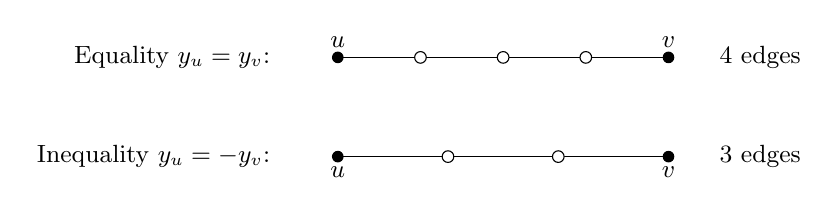
\begin{tikzpicture}[every node/.style={font=\small},scale=1.05]
\node[anchor=east] at (-.7,1.2) {Equality $y_u=y_v$:};
\node[anchor=east] at (-.7,0) {Inequality $y_u=-y_v$:};
\draw (0,1.2) -- (4,1.2);
\draw (0,0) -- (4,0);
\foreach \x in {0,4} {
 \fill (\x,1.2) circle (2pt);
 \fill (\x,0) circle (2pt);
}
\foreach \x in {1,2,3} \draw[fill=white] (\x,1.2) circle (2pt);
\foreach \x in {1.333,2.667} \draw[fill=white] (\x,0) circle (2pt);
\node[above] at (0,1.2) {$u$};
\node[above] at (4,1.2) {$v$};
\node[below] at (0,0) {$u$};
\node[below] at (4,0) {$v$};
\node[anchor=west] at (4.5,1.2) {$4$ edges};
\node[anchor=west] at (4.5,0) {$3$ edges};
\end{tikzpicture}

\caption{Each unit demand becomes a path with fresh internal vertices.
For fixed endpoint signs, its minimum uncut cost is zero if the demand
holds and one otherwise. Identifying the endpoints gives a four-cycle
or a triangle and handles self-demands with the same exact cost.}
\label{fig:paths}
\end{figure}


For an ordinary path with $L$ edges, write the vertex signs along it as
$x_0,\ldots,x_L$, and let $r$ be the number of its uncut edges.
Exactly $L-r$ adjacent pairs have opposite signs. Hence
\begin{equation}\label{eq:path-parity}
 x_0x_L=\prod_{i=1}^L x_{i-1}x_i=(-1)^{L-r}.
\end{equation}
When the prescribed relation holds, alternating signs from the first
endpoint give $r=0$ and reach the prescribed last sign. When it fails,
\eqref{eq:path-parity} rules out $r=0$; making exactly one adjacent
pair equal and alternating on all other edges reaches the prescribed
last sign and gives $r=1$. The same argument with $x_L=x_0$ proves
the assertion for coincident endpoints. A four-cycle has minimum zero,
as required by a self-equality; a triangle has minimum one, as required
by a self-inequality. Thus each gadget has conditional minimum equal
to the failure indicator of its demand.

For any fixed signs on the original vertices, its gadgets can attain
these minima independently because their internal vertices are disjoint.
Conversely any sign assignment on the graph pays at least the sum of
these conditional minima. Minimizing over the original signs and using
\eqref{eq:finite-folding} proves \eqref{eq:exact-graph-optimum}, with
no additive term.

No gadget has a loop or a repeated edge. Within a gadget all its internal
vertices are distinct; the coincident-endpoint cases have lengths at
least three. Between gadgets an edge cannot be repeated, since every
edge contains a vertex internal to its own gadget. The construction
therefore gives a simple undirected graph and assigns every edge unit
weight.

There are at most $2H_KM_0^t$ actual questions, and a constant number
depending only on $K$ of sign variables at each. A gadget introduces at
most three vertices and four edges. Equation~\eqref{eq:total-multiplicity}
therefore proves the stated size bound. All actual questions and query
tables can be identified by deterministic comparisons or sorting of
their canonical encodings. Equality of variable names, construction of
the affine alphabets, and table pullback require a polynomial amount of
work per outer sample; the only unbounded strings are names from the
polynomial-size starting instance. The sample count is polynomial for
fixed $t$. The integers in \eqref{eq:polynomial-denominator} and
\eqref{eq:total-multiplicity} have $O_K(1+\log M_0)$ bits. Explicitly
writing their multiplicities costs $O_K(M_0^t)$ iterations, and vertex
identifiers have $O_K(1+\log M_0)$ bits. These observations include the
cost of constructing the vertex and edge lists and all required integer
arithmetic.
\end{proof}

\subsection{The strict gap and algorithmic consequences}

\begin{proof}[Proof of Theorem~\ref{thm:main}]
Given a $3$SAT instance, perform the deterministic reduction in
Theorem~\ref{thm:max3lin} with the rational completeness error chosen by
Proposition~\ref{prop:bit-gap}. It supplies the nonempty uniform list of
length $M_0$. Carry out Lemmas~\ref{lem:finite-game} and
\ref{lem:graph-realization}, compute $D_0$ by
\eqref{eq:polynomial-denominator}, and output the graph together with
\[
 k=5D_0.
\]
This is a positive integer, computed without knowledge of the optimum.
In the YES case these Lemmas give
\[
 \OPT_{\mathrm{uncut}}(G)<\frac92D_0<5D_0=k.
\]
In the NO case they give
\[
 \OPT_{\mathrm{uncut}}(G)>
       \left(10K-\frac12\right)D_0
       >5KD_0=Kk,
\]
where the second inequality holds for every $K\ge2$.

All parameter searches in the preceding sections use the displayed
effective inequalities. The additional integer searches, rational
integrations, cell enumerations, and sign-table construction in this
Section are also algorithms. The reduction performs this preliminary
work itself; no table or numerical advice is supplied to it. Its cost
is a finite constant for fixed $K$. The starting reduction has
polynomial work and output length, and Lemma~\ref{lem:graph-realization}
establishes polynomial work and output length for every subsequent
step. The integer $k$ has $O_K(1+\log M_0)$ bits. Composition is
therefore a deterministic polynomial-time many-one reduction with all
the graph properties and the strict positive-threshold gap in the
statement.
\end{proof}

For clarity, the deterministic and randomized approximation consequences
are distinct. Let $C>1$ be a fixed real factor and choose a fixed integer
$K\ge\max\{2,C\}$. A deterministic polynomial-time algorithm returning
a bipartition of cost at most $C\OPT_{\mathrm{uncut}}(G)$ would decide
$3$SAT: run it on the output graph and accept exactly when its cut has
cost at most $Kk$. In a YES instance its cost is at most $Ck\le Kk$;
in a NO instance every bipartition costs more than $Kk$. Thus such an
algorithm implies $\mathsf P=\NP$.

If instead a randomized polynomial-time algorithm returns such a
bipartition with probability at least a fixed positive constant, validate
the returned bipartition and apply the same cost check. A NO instance
can never be accepted, regardless of the algorithm's random choices.
A YES instance is accepted whenever the approximation succeeds.
Independent repetition a fixed number of times raises this probability
to at least $1/2$ if necessary. This puts $3$SAT in $\RP$, and composing
with deterministic reductions to $3$SAT gives $\NP\subseteq\RP$.
The randomized conclusion is therefore the latter containment.

\subsection{Minimum 2CNF clause deletion}
\label{sec:2cnf-consequence}

\begin{proof}[Proof of Corollary~\ref{cor:min-2cnf-deletion}]
Given $G=(V,E)$, introduce a variable $x_v$ for each vertex and, for each edge
$uv$, the two clauses
\[
 (x_u\lor x_v),\qquad(\neg x_u\lor\neg x_v).
\]
Call the resulting formula $F_G$. Equal endpoint values falsify exactly one
of these clauses, while unequal values satisfy both. Thus, for every
assignment $a$ and $S_a=\{v:a(x_v)=1\}$,
\[
 \operatorname{unsat}(F_G,a)=\Uncut_G(S_a).
\]
Deleting an assignment's false clauses gives a feasible deletion set of the
same cost. Conversely, from every feasible deletion set $D$, a polynomial-time
$2$SAT algorithm finds an assignment $a$ satisfying $F_G\setminus D$.
Every original clause it falsifies belongs to $D$, so
$\Uncut_G(S_a)=\operatorname{unsat}(F_G,a)\le\abs{D}$. Consequently,
\[
 \OPT_{\rm del}(F_G)=\min_a\operatorname{unsat}(F_G,a)
                  =\OPT_{\rm uncut}(G).
\]

Fix $C>1$ and choose a fixed integer $K\ge\max\{2,C\}$ in
Theorem~\ref{thm:main}. The construction has $\abs{V}$ variables and
$2\abs{E}$ clauses and preserves the gap at the same binary-encoded integer
$k\ge1$: $\OPT_{\rm del}(F_G)\le k$ if the source formula is satisfiable,
and $\OPT_{\rm del}(F_G)>Kk$ otherwise. A $C$-approximation
returns a feasible deletion set with $\abs{D}\le Ck\le Kk$ in the former
case, whereas every feasible deletion set has $\abs{D}>Kk$ in the latter.
Comparing its size with the integer $Kk$ therefore decides $3$SAT in
polynomial time.
\end{proof}

\bibliographystyle{plain}
\bibliography{references}
\end{document}
